\documentclass[12pt, letterpaper]{article}
\usepackage[margin=1.5in]{geometry} % standard is 1.5inch
\usepackage{graphicx}
\usepackage{caption}
\usepackage{amsmath}
\usepackage{amsthm}
\usepackage{bbm}
\usepackage{tikz}
\usepackage[title]{appendix}
\usepackage{hyperref}
\usetikzlibrary{patterns}
%\usepackage{stix}
\usepackage{amssymb}
\usepackage{enumitem}
\title{Thesis Rough Work}
\author{Justin Furlotte (Student \#: 64238736)}
\date{May 17, 2022}
\begin{document}
\begin{titlepage}
\maketitle
\end{titlepage}

\newtheorem{theorem}{Theorem}
\newtheorem{corollary}{Corollary}
\newtheorem{lemma}{Lemma}
\newtheorem{proposition}{Proposition}
\newtheorem{assumption}{Assumption}
 
\newcommand{\C}{\mathbb{C}}
\newcommand{\Tr}{\text{Tr}}
\newcommand{\eps}{\varepsilon}
\newcommand{\R}{\mathbb{R}}
\newcommand{\N}{\mathbb{N}}
\newcommand{\Z}{\mathbb{Z}}
\newcommand{\norm}[1]{\lVert #1 \rVert}
\newcommand{\One}{\mathbbm{1}}
\newcommand{\Var}{\text{Var}}
\newcommand{\F}{\mathcal{F}}
\newcommand{\G}{\mathcal{G}}
\newcommand{\U}{\mathcal{U}}


\graphicspath{ {c:/user/justin/grad school/Thesis} }

\section{Introduction}

\section{Nonnteracting Setting}


Consider the lattice $\Z^2$, on which we define a bulk Hamiltonian $H_B$, whose matrix elements follow a short-range assumption:

\[\sup_{y\in\Z^2}\sum_{x\in\Z^2}|H_B(x,y)|(e^{\mu|x-y|}-1) < \infty\]

for some $\mu>0$. We define the bulk conductivity

\[\sigma_B(\lambda) = -i\Tr(P_\lambda[[P_\lambda,\Lambda_1],[P_\lambda,\Lambda_2]])\]

where $P_\lambda$ is the projection onto the eigenstates of $H_B$ with energy lies in $(-\infty,\lambda)$, and where 

\[\Lambda_i(x) = \begin{cases} 1 & x_i < 0\\ 0 & x_i \geq 0\end{cases}\]

are characteristic functions. We construct an edge Hamiltonian on the lattice $\Z^2_a = \{x \in \Z^2 : x_2 > -a\}$. We denote the edge Hamiltonian by $H_a:\ell^2(\Z^2_a) \to \ell^2(\Z^2_a)$, requiring only that that the edge operator $E_a:\ell^2(\Z^2_a)\to\ell^2(\Z^2_a)$ define by 

\[E_a = J_aH_a-H_BJ_a\]

satisfies the edge assumption

\[\sup_{x\in\Z^2}\sum_{y\in\Z^2_a} E_a(x,y)|e^{\mu(|x_2+a|-|x_1-y_1|)} < \infty\]

for some $\mu>0$, where $|x| := |x_1|+|x_2|$. The interpretation





Each site $x \in \mathbb{Z}^2$ get an associated Hilbert space $\mathcal{H}_x$. The dimension of these Hilbert spaces is bounded uniformly in $x$. We consider the Hilbert space $\ell^2(\mathbb{Z}^2, \mathbb{C}^n) = \{ (x_1,x_2,\ldots) \subset \mathbb{C}^n : \sum_{i \in \Z^2} \norm{x_i}^2 < \infty\}$. For example, one might consider a system of spins at the lattice sites, in which case the Hilbert space $\mathcal{H}_x$ at each site would be $\C^2$, and the total Hilbert space $\mathcal{H} = \otimes_x \mathcal{H}_x$ would then be the space of summable wavefunctions $\psi = \otimes_x\psi_x \in \ell^2(\Z^2,\C^2)$.

The Hilbert space $\ell^2(\Z^2)$ is the ``bulk" setting, i.e. the setting in which we consider an infinite two-dimensional medium with no edges, and we consider a ``bulk Hamiltonian" $H_B$ on this Hilbert space. We also define the ``edge" Hilbert space $\ell^2(\Z_a^2)$ and an associated ``edge Hamiltonian" $H_a$, where $\Z^2_a := \{(n,m) \in \Z^2 : n \geq -a\}$. The bulk and edge Hamiltonians are related by the edge operator $E_a : \ell^2(\Z^2_a) \to \ell(\Z^2)$ defined by

\[E_a := J_aH_a - H_BJ_a,\]

where $J_a : \ell^2(\Z_a^2) \to \ell(\Z^2)$ denotes extension by zeroes. We assume that

\begin{assumption}
The edge operator satisfies
\[\sup_{z\in\Z^2}\sum_{y\in\Z^2_a} |E_a(x,y)| e^{\alpha(|x_2 + a| + |x_1-y_1|)} < \infty\]
for some $\alpha>0$.
\label{ass:edge}
\end{assumption}



The interpretation is that $E_a = J_aH_a - H_BJ_a$ is the difference between first applying $H_a$ on $\ell^2(\Z^2_a)$, and then making everything below $-a$ into zeroes, versus first making all $x \in \Z^2$ such that $x_2 < -a$ zeroes, and the applying $H_B$. The assumption ensures that the effects from introducing the edge at $-a$ die exponentially as we move upward away from the edge (due to the $|x_2 - (-a)|$ term in the exponent), and also terms do not interact too much as their $x_1$ distance increases (due to the $|x_1-y_1|$ term in the exponent).

We also make the following assumption about both the bulk and edge Hamiltonians:

\begin{assumption}
The Hamiltonians have a spectral gap. There exists an interval $\Delta$ such that $\Delta \cap \sigma(H) = \varnothing$.
\end{assumption}

\textit{Remark}: The spectral gap assumption can be relaxed to a ``mobility gap" assumption,
\[\sup_{f \in B_c(\Delta)}|f(H_B)(x,y)|(1+|x|)^{-\nu}e^{\mu|x-y|} < \infty\]
for some $\nu>0$, where $B_c(\Delta)$ is the set of Borel functions $f$ which are constant on $(-\infty,\inf \Delta)$ and on $(\sup \Delta, \infty)$ such that $|f(x)| \leq 1$ for all $x$. See ? for details.

An example of an edge Hamiltonian satisfying the assumption on $E_a$ is $H_a = J_a^*H_BJ_a$, where $J_a:\ell^2(\Z^2_a)\to\ell^2(\Z^2)$ denotes extension by zeros. The idea is that for a state $\psi \in \ell^2(\Z^2_a)$, we have $\langle \psi, H_a \psi \rangle = \langle (J_a \psi), H_B (J_a\psi) \rangle$, which we interpret as the edge Hamiltonian having the same expectation as the bulk Hamiltonian if we just turned all the states $\psi_x$ with $x_2<-a$ into zeroes.  The edge operator is 

\[E_a = J_aJ_a^*H_BJ_a - H_bJ_a = (J_aJ_a^*-\One)H_BJ_a = \begin{cases} -H_B(x,y) & \text{if } x_2 < -a \\ 0 & \text{if } x_2\geq -a\end{cases}\]

Intuitively, there is no difference between $H_B$ and $H_a$ on $\Z^2_a$. The bound in assumption ? is satisfied by the short range assumption ?.

We define the \textit{bulk conductivity} at Fermi energy $\mu$ as follows. Suppose we subject the system to an external electric potential difference $V$ in the $x_2$ direction. We write this as $-V_0 \Lambda_2$, where $\Lambda_i$ are multiplication operators $\Lambda_i |\psi(x_1,x_2)\rangle = \Lambda(x_i)|\psi(x_1,x_2)\rangle$ which are \textit{switch functions},

\[\Lambda : \R\to\R \quad\quad\quad\quad \Lambda(x_i) = \begin{cases} 1 & \text{if } x_i \leq 0 \\ 0 & \text{if } x_i \geq1\end{cases}\]

and are smooth and monotonically decreasing on $(0,1)$. Note that the ensuing physics (in particular, our definition of the Hall conductivity) is independent of the particular choice of switch function $\Lambda_i$, since any two switch functions are exactly equal on the lattice. 

This gives $\vec{E}=-\nabla V = V_0\frac{\partial \Lambda_2}{\partial x_2}$, so that $\vec{E}$ is has compact support $\text{supp}(\Lambda_2')$. We introduce a function which grows slowly in time as $t$ grows from $-\infty$ to 0, so as to invoke the adiabatic principle. Here, we choose $e^{\eps t}$, and we will let $\eps\to 0$ at the end. The Hamiltonian therefore experiences a perturbation, 

\[\widetilde{H}_B(t) = H_B - V_0\Lambda_2 e^{\eps t}.\]

We define the Hall current operator $J_H = i[\widetilde{H}_B(t), \Lambda_1] = i[H_B,\Lambda_1]$, which is related to the Hall conductivity by $J_H = \sigma_H V$. 

\begin{lemma}
The ground state expectation $\Tr(P_\mu J_H)$ of the Hall current is zero.
\end{lemma}
\begin{proof}
Notice that since $J_H$ is trace-class and $P_\mu$ is bounded, and since $[H_B,P_\mu]=0$, we have 

\[\Tr(P_\mu J_H) =i \Tr(P_\mu [H_B, \Lambda_1]) = i\Tr(P_\mu [H_B, P_\mu \Lambda_1P_\mu])\]

\end{proof}

\begin{proposition}

The Hall conductivity $\sigma_H$ in the bulk system is equal to 

\[\sigma_B = -i\emph{Tr}\left(P_\mu \left[[P_\mu,\Lambda_1],[P_\mu,\Lambda_2]\right]\right),\]

where $P_\mu := P((-\infty,\mu))$ is the projection-valued measure associated with $H_B$ onto states with energy less than the Fermi energy $\mu$.
\end{proposition}
\begin{proof}
We begin with the Heisenberg equation of motion for the density matrix, $\dot{\rho}(t) = - i[\widetilde{H}_B(t),\rho(t)]$, with initial condition $\lim_{t\to-\infty} \|\rho(t) - e^{-itH_B}P_\mu e^{itH_B}\| = 0$, which also implies $\lim_{t\to-\infty} \|e^{itH_B}\rho(t)e^{-itH_B} - P_\mu\| = 0$.

We work in the interaction picture, and define $\rho_I(t) = e^{itH_B}\rho(t)e^{-itH_B}$, and $\Delta H_B(t) = -e^{itH_B}V_0\Lambda_2 e^{\eps t}e^{-itH_B}$. Thus

\[\dot{\rho}_I(t) = -i[\Delta H_B(t), \rho_I(t)]\]

The solution to this differential equation is readily verified to be

\[\rho(t) = i\int_{-\infty}^t [\Delta H_B(s), P_\mu]ds + P_\mu \]

Indeed, taking the derivative of the right hand side gives $i[\Delta H_B(t), P_\mu] = i[\Delta H_B(t), \rho_I(t)] + \mathcal{O}(V_0^2)$, but $P_\mu$ and $\rho_I(t)$ are equal up to zeroth order in $V_0$. The initial condition is also satisfied. 

Using $J_H = i[H_B,\Lambda_1] = \sigma_H V = -\sigma_H V_0\Lambda_2$, we obtain $\sigma_H = \frac{1}{V_0} \lim_{\eps\to 0} \Tr(\rho(0)i[H_B,\Lambda_1])$. Since the expectation of the ground state current is zero, $\Tr(P_\mu J_H) =0$, we have

\[\begin{aligned}
\sigma_H &= \frac{i}{V_0} \lim_{\eps\to 0}\Tr \left( i\int_{-\infty}^0 [\Delta H_B(t), P_\mu] [H_B,\Lambda_1] ds\right)\\
&= -\frac{1}{V_0} \lim_{\eps\to 0}\Tr \left( \int_{-\infty}^0 [-e^{isH_B}V_0\Lambda_2 e^{\eps s}e^{-isH_B}, P\mu] [H_B,\Lambda_1] ds\right)\\
&= -\lim_{\eps\to 0}\Tr \left( \int_{-\infty}^0 e^{isH_B}[\Lambda_2, P_\mu]e^{-isH_B}[H_B,\Lambda_1] e^{\eps s}ds\right)\\
&= -\lim_{\eps\to 0}\Tr \left( \int_{-\infty}^0 (e^{-isH_B}[H_B,\Lambda_1]e^{isH_B})\cdot([\Lambda_2, P_\mu] e^{\eps s})ds\right)\\
\end{aligned}\]

Where we used the fact that $P_\mu$ and $H_B$ commute. Using integration by parts on the two terms in brackets, and noting that $\frac{d}{ds}(e^{isH_B}[H_B,\Lambda_1] e^{-isH_B}) = -(ie^{isH_B}\Lambda_1 e^{-isH_B} - \Lambda_1)$, we obtain

\[\begin{aligned}
\sigma_H &= i \lim_{\eps\to 0}\Tr \left( \int_{-\infty}^0 (e^{-isH_B}\Lambda_1e^{isH_B} - \Lambda_1)\frac{d}{ds}([\Lambda_2, P_\mu] e^{\eps s})ds\right)\\
&= i \lim_{\eps\to 0}\eps \Tr \left( \int_{-\infty}^0 \Lambda_1^s[\Lambda_2, P_\mu] e^{\eps s})ds\right)\\
\end{aligned}\]

where $\Lambda_1^s := e^{-isH_B}\Lambda_1e^{isH_B} - \Lambda_1$. Using the notation $\overline{A} := P_\mu AP_\mu^\perp + P_\mu^\perp A P_\mu$, it is readily verified that the commutator $[\Lambda_2, P_\mu]$ is an \textit{off-diagonal} operator, in the sense that  $[\Lambda_2, P_\mu] = \overline{[\Lambda_2,P_\mu]}$. Furthermore, a simple computation reveals that for any two operators $A$ and $B$, $\Tr(\overline{A}B) = \Tr(A\overline{B})$. It therefore follows that

\[\begin{aligned}
\sigma_H &= i \lim_{\eps\to 0}\eps \Tr \left( \int_{-\infty}^0 \overline{\Lambda_1^s}[\Lambda_2, P_\mu] e^{\eps s})ds\right)
\end{aligned}\]

The integrand can be broken into two terms, 

\[\overline{\Lambda_1^s}[\Lambda_2, P_\mu] e^{\eps s} = e^{-isH_B}\overline{\Lambda_1}e^{isH_B}[\Lambda_2, P_\mu]e^{\eps s} - \overline{\Lambda_1}[\Lambda_2, P_\mu]e^{\eps s}\]

by commutativity of $P_\mu$ and $H_B$. We show that the integral of the first term vanishes. We begin by breaking the first term down further into

\[e^{-isH_B}P_\mu \Lambda_1 P_\mu^\perp e^{isH_B}[\Lambda_2, P_\mu]e^{\eps s} + e^{-isH_B}P_\mu^\perp \Lambda_1 P_\mu e^{isH_B}[\Lambda_2, P_\mu]e^{\eps s}.\]

We treat the first of these two terms; the other is handled in an identical manner. We use the spectral theorem to write $e^{-isH_B}P_\mu = \int_{-\infty}^\mu e^{-is\lambda}dP_\lambda$, and similarly $P_\mu^\perp e^{isH_B} = (\text{Id} - P_\mu) e^{isH_B} = \int_\mu^\infty e^{is\nu} dP_\nu$. 

We remark that, since the Fermi energy $\mu$ is assumed to lie in a spectral gap, there must exist a neighbourhood $(\mu-\delta, \mu+\delta)$ in which there are no states. We exploit this fact to rewrite the limits of integration, $\int_{-\infty}^{\mu-\delta} e^{-is\lambda}dP_\lambda$ and $\int_{\mu+\delta}^\infty e^{is\nu} dP_\nu$. We therefore obtain

\[\begin{aligned} 
\lim_{\eps\to 0} &\eps \int_{-\infty}^0 e^{-isH_B}P_\mu \Lambda_1 P_\mu^\perp e^{isH_B}[\Lambda_2, P_\mu]e^{\eps s} ds \\
&\quad\quad= \lim_{\eps\to 0} \eps \Tr\left( \int_{-\infty}^0 \int_{-\infty}^{\mu-\delta} e^{-is\lambda}dP_\lambda \Lambda_1 \int_{\mu+\delta}^\infty e^{is\nu} dP_\nu [\Lambda_2, P_\mu] e^{\eps s} ds\right)\\
&\quad\quad= \lim_{\eps\to 0} \eps \Tr\left( \int_{-\infty}^0 \int_{-\infty}^{\mu-\delta} \int_{\mu+\delta}^\infty e^{s(\eps-i\lambda+i\nu)}dP_\lambda \Lambda_1 dP_\nu [\Lambda_2, P_\mu]ds\right)\\
\end{aligned}\]

Performing the integral over $s$ yields

\[\lim_{\eps\to 0}\eps \int_{-\infty}^0 e^{s(\eps-i\lambda+i\nu)}ds = -\lim_{\eps\to 0} \frac{\eps}{i\eps + \lambda-\nu}\]

This limit is zero, since $\lambda \neq \nu$. Indeed, due to the spectral gap, the integration variables live in $\lambda \in (-\infty, \mu-\delta)$ and $\nu \in (\mu+\delta,\infty)$. The case for the $e^{-isH_B}P_\mu^\perp \Lambda_1 P_\mu e^{isH_B}[\Lambda_2, P_\mu]e^{\eps s}$ term (where the $P_\mu$ and $P_\mu^\perp$ swap places) is treated analogously. Hence the first term in the integrand for $\sigma_H$ vanishes, as claimed. 

Finally, we return to our expression for the Hall conductivity, which now reads

\[\sigma_H = i\lim_{\eps\to 0}\eps \Tr\left(\int_{-\infty}^0 \overline{\Lambda_1}[\Lambda_2, P_\mu]e^{\eps s}ds\right).\]

It is a basic algebraic calculation to show that $\overline{\Lambda_1} = [[\Lambda_1, P_\mu],P_\mu]$. Evaluating the integral over $s$ is now trivial; $\int_{-\infty}^0 e^{\eps s}ds = \eps^{-1}$. Thus

\[\sigma_H = -i\Tr([[\Lambda_1,P_\mu],P_\mu][\Lambda_2,P_\mu]).\]

Shifting the commutator completes the proof:

\[\begin{aligned}
\sigma_H &= -i\Tr(P_\mu[[\Lambda_2,P_\mu],[\Lambda_1,P_\mu]]) \\
&= i\Tr(P_\mu[[\Lambda_1,P_\mu],[\Lambda_2,P_\mu]])\\
&= i\Tr(P_\mu[[P_\mu,\Lambda_1],[P_\mu,\Lambda_2]]).
\end{aligned}\]

\end{proof}

\textit{Remark:} This is reminiscent of the well-known adiabatic curvature formula,

\[\kappa = \Tr(P[\partial_1P,\partial_2 P]) = \Tr(P\left[ [P,K_1], [P,K_2] \right]) = \Tr(P[K_1,K_2]),\]

where $K_i$ are called \textit{generators of parallel transport}. We will see the adiabatic curvature formula again later in the interacting setting. 

For the \textit{edge conductivity}, we need the current operator across the line $x_1=0$, which is given by $-i[H_a,\Lambda_1]$. We define 

\[\sigma_E = -i\lim_{a\to\infty}\Tr(\rho'(H_a)[H_a,\Lambda_1]),\]

where $\rho \in C^\infty(\R)$ satisfies

\[\rho(r) = \begin{cases} 1 & \text{if } r<\inf\Delta\\ 0 & \text{if } r>\sup\Delta\end{cases}\]

and decreases smoothly and monotonically in $\Delta$. The definition of $\sigma_E$ is reminiscent of another formula we will see later in the interacting setting, $\Tr(\dot{P}J)$, where $J$ is the current operator. The interpretation of $\sigma_E$ is that if we apply a small potential difference $V$ across $x_2=-a$ to $x_2=\infty$, there will be a net current

\[\begin{aligned}
I &= -i\Tr(\rho(H_a+V)[H_a+V,\Lambda_1] - \rho(H_a)[H_a,\Lambda_1])\\
&= -i\Tr((\rho(H_a+V)-\rho(H_a))[H_a,\Lambda_1])
\end{aligned}\]

Thus we obtain the conductivity

\[\sigma_E = \frac{I}{V} = -i\Tr\left(\frac{(\rho(H_a+V)-\rho(H_a)}{V}[H_a,\Lambda_1]\right) \to -i\Tr(\rho'(H_a)[H_a,\Lambda_1])\]

in the limit as $V\to0$. As we shall see, it turns out that $\sigma_E$ is independent of the choice of $\rho$, and $\sigma_B$ is independent of $\lambda$. 

The main result of this section is

\begin{theorem}
$\sigma_E=\sigma_B$.
\end{theorem}

\subsection{Outline of the Proof}

First, let 

\[\tilde{\sigma}_E(a,t) = -i\Tr(\rho'(H_a)[H_a,\Lambda_1]\Lambda_{2,a}(t))\]

where $\Lambda_{2,a}(t) = e^{itH_a}\Lambda_2 e^{-itH_a}$ is the time evolution of $\Lambda_2$. One can show that, while 

\[\sigma_E = \lim_{T\to\infty}\lim_{a\to\infty} \frac{1}{T}\int_0^T \text{Re}(\tilde{\sigma}_E(a,t))dt,\]

it is unfortunately the case that $\lim_{a\to\infty}\norm{\rho'(H_a)[H_a,\Lambda_1]\Lambda_{2,a}(t)}_1 = \infty$. However, even though the trace norm diverges, it turns out that the trace itself does not, so we will instead subtract a clever choice of zero-trace operator $Z(a,t)$ to define

\[\sigma_E(a,t) = -i\Tr(\rho'(H_a)[H_a,\Lambda_1]\Lambda_{2,a}(t)-Z(a,t))\]

so that the equation $\sigma_E = \lim_{T\to\infty}\lim_{a\to\infty} \frac{1}{T}\int_0^T \text{Re}(\sigma_E(a,t))dt$ still holds, but we also have $\lim_{a\to\infty}\norm{\rho'(H_a)[H_a,\Lambda_1]\Lambda_{2,a}(t) - Z(a,t)}_1 < \infty$. The correct choice of $Z$ will become apparent after writing $\rho(H_a)$ and $\rho'(H_a)$ in terms of their Hellfer-Sj\"{o}strand representations,

\[\rho(H_a) = \frac{1}{2\pi} \int_\C \frac{\partial \tilde{\rho}(z)}{\partial \bar{z}} R(z)\]

\[\rho'(H_a) = -\frac{1}{2\pi}\int_\C \frac{\partial \tilde{\rho}(z)}{\partial \bar{z}} R(z)^2\]

where $R(z) = (H_a - z)^{-1}$ is the resolvent. Using $[R(z),\Lambda_i] = R(z)[H_a,\Lambda_i]R(z)$, we obtain the representations of the following useful operators:

\[[\rho(H_a),\Lambda_1] = \frac{1}{2\pi} \int_\C \frac{\partial \tilde{\rho}(z)}{\partial \bar{z}} R(z)[H_a,\Lambda_1]R(z)\]

\[\rho'(H_a)[H_a,\Lambda_1] = -\frac{1}{2\pi} \int_\C \frac{\partial \tilde{\rho}(z)}{\partial \bar{z}} R(z)^2[H_a,\Lambda_1]\]

From here, we define the zero-trace operator

\[Z(a,t) = [\rho(H_a),\Lambda_1]\Lambda_2 - \frac{1}{2\pi} \int_\C \frac{\partial \tilde{\rho}(z)}{\partial \bar{z}} R(z)(R(z)[H_a,\Lambda_1]\Lambda_{2,a}(t) - [H_a,\Lambda_1]\Lambda_{2,a}(t)R(z))\]

from which we obtain

\[\begin{aligned}
\sigma_E(a,t) &= \tilde{\sigma}_E(a,t) - Z(a,t)\\
&= \Tr\left(-[\rho(H_a),\Lambda_1]\Lambda_2 - \frac{1}{2\pi}\int_\C \frac{\partial \tilde{\rho}(z)}{\partial \bar{z}}R(z)[H_a,\Lambda_1]\Lambda_{2,a}(t)R(z)\right)\\
&= \Tr\left([\rho(H_a),\Lambda_1](\Lambda_{2,a}(t)-\Lambda_2) - \frac{1}{2\pi}\int_\C\frac{\partial \tilde{\rho}(z)}{\partial \bar{z}}R(z)[H_a,\Lambda_1]R(z)[H_a,\Lambda_{2,a}(t)]R(z)\right)
\end{aligned}\]

All of the statements so far can be verified by calculations. The difficult part of the theorem (aside from proving that the relevant operators are trace-class) is proving that

\[\norm{J_a\Sigma_a'J_a^* - \Sigma_B'}_1, \norm{J_a\Sigma_a''J_a^* - \Sigma_B''}_1 \to 0\]

as $a\to\infty$, where $\Sigma_B'$ and $\Sigma_B''$ are the same as with the subscript $a$, except using the bulk Hamiltonian $H_B$ in their definition rather than $H_a$. It follows that 

\[\sigma_E(a,t) = \Tr(J_a\Sigma_a'J_a^*+J_a\Sigma_a''J_a^*) = \Tr(\Sigma_a'+\Sigma_a'') \to \Tr(\Sigma_B'+\Sigma_B'')\]

From there, a calculation shows that $\lim_{T\to\infty}\frac{1}{T}\int_0^T\Tr(\Sigma_B'+\Sigma_B'')dt = \sigma_B$, concluding the proof.

\subsection{Gap Simplifications}

We now assume that $H_B$ has a spectral gap. In this case, the edge condition guarantees that $\sigma_E(a) := \rho'(H_a)[H_a,\Lambda_1]$ is trace-class (need to add). 

Need to add section on why $\sigma_E(a) := -i\Tr(\rho'(H_a)[H_a,\Lambda_1])$ is equal to

\[-\frac{i}{2}\Tr(\rho'(H_a)\{[H_a,\Lambda_1],\Lambda_2\}).\]

\begin{theorem}
$\sigma_E = \sigma_B$
\end{theorem}

\subsubsection*{Outline of the Proof}

Before giving the proof in its entirety, we outline the basic steps. The key ingredient is the use of the funcional calculus given by the Helffer-Sj\"{o}strand representation of self-adjoint operators on a Hilbert space (need to add reference to appendix here).

\subsection*{The Proof}

\begin{proof}

We posit that the edge conductivity can be rewritten as $\sigma_E = \lim_{a\to\infty}\sigma_E(a)$, where

\[\sigma_E(a) = -i\Tr(\rho'(H_a)[H_a,\Lambda_1]\Lambda_2),\]

since we have assumed that there is a spectral gap (as opposed to a mobility gap), so that there are extended states near the edge, and no bound states or resonances far from the edge. Thus, intuitively, the cutoff introduced by $\Lambda_2$ is irrelevant as we take $a\to\infty$. We provide a more concrete justification for this later.


\textit{``Concrete justificiation":}
Since $\sigma_B$ is translation invariant (need to add), we only need to prove to case $-i\Tr(\rho'(H_{a=0})[H_{a=0},\Lambda_1] = \sigma_B$. We drop the subscript, $H := H_{a=0}$. Since the multiplication operator $\Lambda_2(n) |\psi\rangle := \Lambda(x_2-n) |\psi\rangle$ converges strongly to the identity as $n\to\infty$, we can write

\[\sigma_E(a) = -i\Tr(\rho'(H)[H,\Lambda_1]) = -i\lim_{n\to\infty}\Tr(\rho'(H)[H,\Lambda_1]\Lambda_2(n)).\]

Instead of completing the shift $(0,-n)$ with the operator $\Lambda_2(n)$, we can consider a shifted Hamiltonian. Indeed, rather than restrict $H_B$ at $x_2=-n$ to obtain $H_{a=n}$, consider the shifted bulk Hamiltonian $H_B \mapsto H_B(n)$ obtained by the shift $(0,-n)$, and then restricting this at $x_2=0$ to obtain $H(n)$. In other words, $H(n)$ is the edge Hamiltonian associated with the shifted bulk Hamiltonian. Comparing this with the expression above, this is exactly equivalent to 

\[-i\lim_{n\to\infty}\Tr(\rho'(H)[H,\Lambda_1]\Lambda_2(n)) = -i\lim_{n\to\infty}\Tr(\rho'(H(n))[H(n),\Lambda_1]\Lambda_2).\]

In other words, the difference between whether we cut off everything above $x_2=n$ and then apply $H_{a=0}$, or instead cut off everything above $x_2=0$ and then apply the Hamiltonian $H(n)$ shifted down by $(0,-n)$ is immaterial. 

Thus, our goal is to show that $-i\Tr(\rho'(H(n))[H(n),\Lambda_1]\Lambda_2) \to \sigma_B$ as $n\to\infty$. 

\textit{End of concrete justification.}

%Notice that the complex conjugate is 

%\[\overline{\widetilde{\sigma_E}(a)} = -i\Tr(\Lambda_2[H_a,\Lambda_1]\rho'(H_a)) = -i\Tr(\rho'(H_a)\Lambda_2[H_a,\Lambda_1])\]

%so that $\sigma_E(a) = \text{Re}(\widetilde{\sigma_E}(a))$. Now, let

Define 

\[ Z(a) = [\rho(H_a),\Lambda_1]\Lambda_2 - \frac{1}{2\pi}\int_\C \frac{\partial \tilde{\rho}}{\partial \bar{z}} R_a(z)[R_a(z),[H_a,\Lambda_1]\Lambda_2] dz^2 \]

This operator has zero trace. Indeed, the first term has vanishing trace in the position basis, while the second term's integrand involves the trace of $[R,R]=0$. The bounds necessary for shifting the commutator like this are on 

\[\norm{R[H_a,\Lambda_1]e^{\delta |x_1|}}, \quad \norm{e^{-\delta |x_1|}e^{-\delta|x_2}}_1, \quad \norm{\Lambda_2 R e^{\delta |x_2|}},\]

the first two of which are given below, and the third is obvious since $\norm{R}$ is bounded and $\Lambda_2$ provides a cutoff which ensures $e^{\delta|x_2|}$ is finite. So $\sigma_E(a) = \Tr(\Sigma(a))$, where

\[\begin{aligned}
\Sigma(a) &=  -i\rho'(H_a)[H_a,\Lambda_1]\Lambda_2 + iZ(a)\\
&= -i\rho'(H_a)[H_a,\Lambda_1]\Lambda_2 + i[\rho(H_a),\Lambda_1]\Lambda_2 - \frac{i}{2\pi}\int_\C\frac{\partial \tilde{\rho}}{\partial \bar{z}} R_a(z)[R_a(z),[H_a,\Lambda_1]\Lambda_2] dz^2.
\end{aligned}\]

Using the Hellfer-Sj\"{o}strand representations for the first two terms on the right hand side, we obtain

\[\begin{aligned}
\Sigma(a) &= \frac{i}{2\pi}\int_\C \frac{\partial \tilde{\rho}}{\partial\bar{z}} R_a(z)^2[H_a,\Lambda_1]\Lambda_2 dz^2 + \frac{i}{2\pi}\int_\C\frac{\partial \tilde{\rho}}{\partial\bar{z}} R_a(z)[H_a,\Lambda_1]R_a(z)\Lambda_2dz^2 \\
&\quad\quad\quad\quad - \frac{i}{2\pi}\int_\C \frac{\partial \tilde{\rho}}{\partial\bar{z}} (R_a(z)^2[H_z,\Lambda_1]\Lambda_2 - R_a(z)[H_a,\Lambda_1]\Lambda_2 R_a(z)) dz^2\\
&= -\frac{i}{2\pi}\int_\C\frac{\partial \tilde{\rho}}{\partial\bar{z}} R_a(z)[H_a,\Lambda_1][R_a(z),\Lambda_2]dz^2\\
&= \frac{i}{2\pi}\int_\C \frac{\partial \tilde{\rho}}{\partial \bar{z}} R_a(z)[H_a,\Lambda_1]R_a(z)[H_a,\Lambda_2]R_a(z) dz^2,
\end{aligned}\]

where we used 

\[[R_a(z),\Lambda_i] = -R_a(z)[H_a,\Lambda_i]R_a(z)\]

in the final equality. Next, we must prove that the operator above converges to the corresponding bulk operator in trace-norm,

\[ \norm{\Sigma(a) - \Sigma_B}_1 \to 0,\]

as $a\to\infty$, which in turn proves that $\Tr(\Sigma(a))\to\Tr(\Sigma_B)$ because of the bound $|\Tr(A)|\leq \norm{A}_1$. Here, $\Sigma_B$ is the same operator as before, but using the bulk operators $H_B$ and $R_B(z)$. Once this limit is established, we shall prove that $\sigma_B = \Tr(\Sigma_B)$ to conclude the proof. 

To show that the limit is zero as claimed, we bound the trace norm of the integrand of $\Sigma(a)$ by breaking it into three parts,

\[R[H_a,\Lambda_1]R[H_a,\Lambda_2]R = J_a[R,\Lambda_1]e^{\delta|x_1|}J_a^*\cdot e^{-\delta|x_1|}e^{-\delta|x_2|}\cdot J_ae^{\delta|x_2|}[H_a, \Lambda_2]RJ_a^*,\]

and bounding the norm of each, making use of the fact that $\norm{AB}_1 \leq \norm{A}\norm{B}_1$.

\begin{enumerate}
\item For the first term, $J_a[R,\Lambda_1]e^{\delta|x_1|}J_a^*$, we bound its operator norm by breaking it down further into

\[\begin{aligned}
\|J_a[R,\Lambda_1]e^{\delta|x_1|}J_a^*\| &= \|[R,\Lambda_1]e^{\delta|x_1|}\| \\
&=\norm{-R[H_a,\Lambda_1]Re^{\delta|x_1|}}\\
&= \norm{-R\cdot [H_a,\Lambda_1]e^{\delta|x_1|}\cdot e^{-\delta|x_1|} R e^{\delta|x_1|}}\\
&\leq \norm{R}\cdot \norm{[H_a,\Lambda_1]e^{\delta|x_1|}}\cdot \norm{e^{-\delta|x_1|}Re^{\delta|x_1|}}
\end{aligned}\]

The norm of $R$ is bounded by 

\[\norm{R_a(z)} \leq \frac{1}{|\text{Im}(z)|}\]

for any $z\notin \R$ since $H_a$ is self-adjoint. The norm of the second operator can be bounded by inspecting its matrix elements.

\[\begin{aligned}
\langle x, [H_a,\Lambda_1]e^{\delta|x_1|} y\rangle &= \langle x, H_a\Lambda_1 y\rangle e^{\delta |y_1|} - \langle x, \Lambda_1 H_a y\rangle e^{\delta|y_1|}  \\
&= H_a(x,y)e^{\delta|y_1|}(\Lambda(y_1)-\Lambda(x_1)).
\end{aligned}\]

This is zero if $|x_1-y_1|\leq |y_1|$, since this would imply that $x_1$ and $y_1$ have the same sign, yielding $\Lambda(x_1)=\Lambda(y_1)$. So either the matrix element is zero, or $|y_1|\leq|x_1-y_1|$, which implies

\[\begin{aligned}
|H_a(x,y)e^{\delta|y_1|}(\Lambda(y_1)-\Lambda(x_1))| &\leq 2|H_a(x,y)|e^{\delta|x_1-y_1|}\\
&\leq 2|H_a(x,y)|e^{\delta|x-y|}\\
&\leq C|H_a(x,y)|(e^{\delta|x-y|}-1)
\end{aligned}\]

where the final inequality comes from the fact that the diagonal matrix elements are zero. Hence the assumption 

\[\sup_{x\in\Z^2}\sum_{y\in\Z^2}|H(x,y)|(e^{\mu|x-y|}-1)<\infty,\]

combined with Holmgren's bound

\[\norm{A} \leq \max \left\{ \sup_{x\in\Z^2} \sum_{y\in\Z^2} |A(x,y)|, \; \sup_{y\in\Z^2}\sum_{x\in\Z^2}|A(x,y)| \right\},\]

implies that the second term is bounded. Finally, for the third term $e^{-\delta|x_1|}Re^{\delta|x_1|}$, we apply the Combes-Thomas bound,

\[\norm{e^{-\eps f(x)}R_a(z)e^{\eps f(x)}} \leq \frac{C}{|\text{Im}(z)|}\]

where $f:\Z^2\to\R$ is any Lipschitz function, and $\eps$ can be chosen as $\eps = \frac{1}{C(1+|\text{Im}(z)|)}$.

Altogether, the bound of the first term takes the form 

\[\frac{C}{\text{Im}(z)^2}.\]

\item For $e^{-\delta|x_1|}e^{-\delta|x_2|}$, we bound the trace norm by noticing that this is a positive operator satisfying 

\[\langle (n,m), e^{-\delta|x_1|}e^{-\delta|x_2|} (n,m) \rangle = \langle e^{-\delta|x_1|}e^{-\delta|x_2|}(n,m), (n,m) \rangle,\]

so that its trace norm is equal to its trace. In the position basis, we see that its trace is given by a geometric series

\[\begin{aligned}
\Tr(e^{-\delta|x_1|}e^{-\delta|x_2|}) &= \sum_{(n,m)\in\Z^2} \langle (n,m), e^{-\delta|x_1|}e^{-\delta|x_2|} (n,m) \rangle \\
&\leq 2 \sum_{n=0}^\infty \sum_{m=0}^\infty e^{-\delta m}e^{-\delta n} \\
&= 2\left(\frac{1}{1-e^{-\delta}}\right)^2.
\end{aligned}\]

\item For $J_a e^{\delta|x_2|} [H_a,\Lambda_2] R_a(z)J_a^*$, note that analogously to 1. above where we bounded $[H_a,\Lambda_1]e^{\delta|x_1|}$, we also have that $e^{\delta|x_2|}[H_a,\Lambda_2]$ is bounded. Again, the resolvent $R_a(z)$ is also bounded.

The bound of the third term takes the same form as the bound of the first term,

\[\frac{C}{\text{Im}(z)^2}.\]

\end{enumerate}

Altogether, we see that the integrand is bounded by the product of the three bounds from 1., 2., and 3., and is of the form $\frac{C}{\text{Im}(z)^4}$. 

For any $n\in \N$, the quasi-analytic extension $\tilde{\rho}$ of $\rho$ in the Helffer-Sj\"{o}strand representation can be chosen so that 

\[\int_\C\frac{\partial \tilde{\rho}}{\partial \bar{z}} \frac{1}{|\text{Im}(z)|^{p+1}}dz^2 \leq C_0 \sum_{k=0}^{n+2 }\norm{\rho^{(k)}}_{k-p-1},\]

where the norms on the right hand side are defined by 

\[\norm{f}_{m} = \int_{-\infty}^\infty |f(x)|(x^2+1)^{m/2}dx.\]

Since $|\rho(x)|\leq 1$ and $\rho'$ is compactly supported, these norms are all clearly finite. This fact, combined with the bound 

\[\norm{R_a(z)[H_a,\Lambda_1]R_a(z)[H_a,\Lambda_2]R_a(z)}_1 \leq \frac{C}{\text{Im}(z)^4}\]

for the trace norm of the integrand of $\Sigma(a)$ provides the necessary bound for Lebesgue dominated convergence. Thus, it suffices to show pointwise convergence in $z$ of the integrand to the associated bulk operator. 

In other words, we wish to show 

\[ J_a[R_a(z),\Lambda_1]e^{\delta|x_1|}J_a^* \xrightarrow{\enskip s \enskip} [R_B(z), \Lambda_1]e^{\delta|x_1|},\]

\[J_ae^{\delta|x_2|}[H_a,\Lambda_2]J_a^* \xrightarrow{\enskip s \enskip} e^{\delta|x_2|}[H_B, \Lambda_2],\]

and 

\[J_aR_a(z)J_a^* \xrightarrow{\enskip s \enskip} R_B(z)\]

for each fixed $z\in\C$. Inspecting the bounds we found for the left hand sides of these limits, it is clear that they are uniformly bounded in $a$. It therefore suffices to show convergence on a dense subspace of $\ell^2(\Z^2)$; in particular, we may choose the dense subspace of compactly supported states, which allows us to ignore the $e^{\delta|x_i|}$ terms. Thus, we need to prove 

\[ J_a[R_a(z),\Lambda_1]J_a^* \xrightarrow{\enskip s \enskip} [R_B(z), \Lambda_1],\]

\[J_a [H_a,\Lambda_2]J_a^* \xrightarrow{\enskip s \enskip} [H_B, \Lambda_2],\]

and 

\[J_aR_a(z)J_a^* \xrightarrow{\enskip s \enskip} R_B(z).\]

In fact, the final statement implies the first two; we appeal to the general fact of functional analysis that strong convergence of the resolvent of a self-adjoint operator implies that $J_a f(H_a) J_a^* \xrightarrow{\enskip s \enskip} f(H_B)$ for any bounded and continuous function $f$. In particular, the functions $[(\cdot - z)^{-1}, \Lambda_1]$ and $[\cdot, \Lambda_2]$ above are bounded and continuous, so we will have proven the desired limits if we can prove the strong convergence of the resolvent, $J_aR_a(z)J_a^* \xrightarrow{\enskip s \enskip} R_B(z)$.

To prove this, we use the edge assumption. Recall the edge operator, $E_a = J_aH_a - H_BJ_a$. Adding and subtracting $zJ_a$ gives

\[E_a = J_a(H_a-z) - (H_B-z)J_a.\]

Applying $R_B$ from the left and $R_a$ from the right on both sides, we obtain 

\[R_B(z)E_aR_a(z) = R_B(z)J_a - J_aR_a(z).\]

Taking the adjoint, and then multiplying from the left by $J_a$, we see that 

\[J_aR_a(z)E_a^*R_B(z) = J_aJ_a^*R_B(z) - J_aR_a(z)J_a^*.\]

Thus

\[R_B(z) - J_aR_a(z)J_a^* = (J_aR_a(z)E_a^* - J_aJ_a^* + 1)R_B(z)  \xrightarrow{\enskip s \enskip} 0,\]

since $E^*_a \xrightarrow{\enskip s \enskip} 0$ by Lemma \ref{lemma:edge}, and $- J_aJ_a^* + 1 \xrightarrow{\enskip s \enskip}  0$. This proves that the limits above converge to the desired associated bulk operators, and hence $\norm{\Sigma(a) -  \Sigma_B}_1 \to 0$.

Finally, it remains to show that  

\[\Tr(\Sigma_B) = \sigma_B.\]

First, we manipulate

\[\begin{aligned}
\Sigma_B &= \frac{i}{2\pi}\int_\C \frac{\partial \tilde{\rho}}{\partial\bar{z}} R_B(z)[H_B,\Lambda_1]R_B(z)[H_B,\Lambda_2]R_B(z) dz^2\\
&= -\frac{i}{2\pi}\int_\C \frac{\partial \tilde{\rho}}{\partial\bar{z}} R_B(z)[H_B,\Lambda_1][R_B(z),\Lambda_2]dz^2\\
&= i[\rho(H_B),\Lambda_1]\Lambda_2 - \frac{i}{2\pi}\int_\C \frac{\partial \tilde{\rho}}{\partial\bar{z}} R_B(z)[H_B,\Lambda_1]\Lambda_2 R_B(z)dz^2.
\end{aligned}\]

Define $P_+ := P((\sup \Delta, \infty))$ and $P_- := P((-\infty, \inf \Delta))$, the projections onto states above and below the gap, respectively. Since $H_B$ is assumed to have a gap, we have 

\[\Tr(\Sigma_B) = \Tr(P_+\Sigma_B P_+) + \Tr(P_-\Sigma_B P_-).\]

Since $P_\pm R_B(z)$ and $R_B(z) P_\pm$ are analytic on $\text{supp}(\rho(z))$ and $\text{supp}(1-\rho(z))$, the integral in $P_\pm \Sigma_B P_\pm$ vanishes by integration by parts. Thus

\[\Sigma_B = iP_+[\rho(H_B),\Lambda_1]\Lambda_2P_+ + iP_-[\rho(H_B),\Lambda_1]\Lambda_2P_-.\]

By the spectral theorem for projection-valued measures, if the Fermi energy lies in the gap, $\lambda \in \Delta$, we have

\[ \rho(H_B) = \int_{-\infty}^\infty \rho(\lambda) dP_\nu = \int_{-\infty}^\lambda \rho(\lambda) dP_\nu = \int_{-\infty}^\lambda dP_\nu = P_\lambda.\]

We may therefore replace $\rho(H_B)$ by $P_\lambda$, by which we obtain

\[\Tr(\Sigma_B) = i\Tr(P_+[P_\lambda,\Lambda_1]\Lambda_2P_+) + i\Tr(P_-[P_\lambda,\Lambda_1]\Lambda_2P_-).\]

Now, the bulk conductivity is given by

\[\begin{aligned}
\sigma_B &= i\Tr(P_\lambda [[P_\lambda, \Lambda_1],[P_\lambda,\Lambda_2]])\\
&= i\Tr(P_\lambda ((P_\lambda \Lambda_1-\Lambda_1P_\lambda)(P_\lambda\Lambda_2 - \Lambda_2P_\lambda) - (P_\lambda\Lambda_2 - \Lambda_2P_\lambda)(P_\lambda\Lambda_1-\Lambda_1P_\lambda)))\\
&= i\Tr(P_\lambda(P_\lambda\Lambda_1P_\lambda\Lambda_2 - P_\lambda\Lambda_1\Lambda_2 P_\lambda - \Lambda_1P_\lambda\Lambda_2 + \Lambda_1P_\lambda\Lambda_2P_\lambda \\
&\quad\quad\quad\quad - P_\lambda\Lambda_2P_\lambda\Lambda_1 + P_\lambda\Lambda_2\Lambda_1P_\lambda + \Lambda_2P_\lambda\Lambda_1 - \Lambda_2P_\lambda\Lambda_1P_\lambda))\\
&= i\Tr(- P_\lambda\Lambda_1\Lambda_2 P_\lambda + \Lambda_1P_\lambda\Lambda_2P_\lambda + P_\lambda\Lambda_2\Lambda_1P_\lambda - \Lambda_2P_\lambda\Lambda_1P_\lambda)\\
&= i\Tr(- P_\lambda\Lambda_1\Lambda_2 P_\lambda + P_\lambda\Lambda_1P_\lambda\Lambda_2P_\lambda + P_\lambda\Lambda_2\Lambda_1P_\lambda - P_\lambda\Lambda_2P_\lambda\Lambda_1P_\lambda)\\
&= i\Tr(P_\lambda\Lambda_1 P_\lambda^\perp \Lambda_2P_\lambda - P_\lambda\Lambda_2 P_\lambda^\perp \Lambda_1 P_\lambda)\\
&= i\Tr(P_\lambda\Lambda_1 P_\lambda^\perp \Lambda_2P_\lambda -  P_\lambda^\perp \Lambda_1 P_\lambda\Lambda_2)\\
&= i\Tr(P_\lambda\Lambda_1 P_\lambda^\perp \Lambda_2P_\lambda -  P_\lambda^\perp \Lambda_1 P_\lambda\Lambda_2P_\lambda^\perp).
\end{aligned}\]

We define $T_\lambda := P_\lambda\Lambda_1 P_\lambda^\perp \Lambda_2P_\lambda -  P_\lambda^\perp \Lambda_1 P_\lambda\Lambda_2P_\lambda^\perp$, so that

\[\sigma_B = i\Tr(T_\lambda),\]

and show that $P_\pm T_\lambda P_\pm = P_\pm [P_\lambda, \Lambda_1]\Lambda_2 P_\pm$. 

First, notice that because of the gap, we have $P_\lambda^\perp P_- = 0$, and thus also $P_\lambda P_- = P_-$. Thus

\[\begin{aligned}
P_- T_\lambda P_- &=  P_-P_\lambda \Lambda_1 P_\lambda^\perp \Lambda_2 P_\lambda P_-\\
&= P_-(P_\lambda\Lambda_1\Lambda_2 - \Lambda_1P_\lambda\Lambda_2)P_-\\
&= P_-[P_\lambda,\Lambda_1]\Lambda_2 P_-,
\end{aligned}\]

and similarly, for $P_+$, we have $P_\lambda^\perp P_+ = P_+$, and $P_\lambda P_- = 0$, which implies

\[\begin{aligned}
P_+ T_\lambda P_+ &=  -P_+P_\lambda^\perp \Lambda_1 P_\lambda \Lambda_2 P_\lambda^\perp P_+\\
&= -P_+P_\lambda^\perp\Lambda_1P_\lambda\Lambda_2P_+\\
&= -P_+P_\lambda^\perp\Lambda_1\Lambda_2P_+ + P_+P_\lambda^\perp\Lambda_1P_\lambda^\perp\Lambda_2P_+\\
&= -P_+P_\lambda^\perp\Lambda_1\Lambda_2P_+ + P_+\Lambda_1P_\lambda^\perp\Lambda_2P_+\\
&= -P_+[P_\lambda^\perp, \Lambda_1]\Lambda_2 P_+\\
&= -P_+[(1-P_\lambda), \Lambda_1]\Lambda_2 P_+\\
&= P_+[P_\lambda, \Lambda_1]\Lambda_2 P_+.
\end{aligned}\]

Finally, we obtain

\[\begin{aligned}
\sigma_B &= i\Tr(T_\lambda) \\
&=  i\Tr(P_-T_\lambda P_-) + i\Tr(P_+T_\lambda P_+)\\
&= i\Tr(P_-[P_\lambda,\Lambda_1]\Lambda_2 P_-) + i\Tr(P_+[P_\lambda, \Lambda_1]\Lambda_2 P_+)\\
&= \Tr(\Sigma_B),
\end{aligned}\]

concluding the proof.
\end{proof}

\begin{lemma}
$E_a$ and $E_a^*$ converge strongly to zero in the limit $a\to\infty$.
\label{lemma:edge}
\end{lemma}
\begin{proof}
Let $\psi \in \ell^2(\Z^2)$. Since $E_a$ has real entries,

\[\begin{aligned}
\norm{E_a^* \psi}^2 &= \langle E_a^*\psi, E_a^* \psi \rangle\\
&=\sum_z \left(\sum_y \overline{E_a^*(z,y)\psi(y)}\right) \left(\sum_x E_a^*(z,x)\psi(x)\right)\\
&=\sum_{z} \left(\sum_y E_a(y,z)\overline{\psi(y)}\right) \left(\sum_x E_a(x,z)\psi(x)\right)\\
\end{aligned}\]

Consider the $M_\alpha(z) := \sum_x E_a(x,z)\psi(x)$ term. To take advantage of the edge assumption, we insert the exponentials

\[M_\alpha(z) = \sum_x E_a(x,z)e^{\alpha (|z_2-a|-|z_1-x_1|)} e^{-\alpha (|z_2-a|-|z_1-x_1|)}\psi(x).\]

By assumption \ref{ass:edge}, $E_a(x,z)e^{\alpha (|z_2-a|-|z_1-x_1|)}$ is bounded uniformly in $x$. Writing $g(z)$ for this bound,

\[M_\alpha(z) \leq g(z) \sum_x e^{-\alpha (|z_2-a|-|z_1-x_1|)}\psi(x).\]

Precisely the same argument can be used on the other term, $N_\alpha(z) \leq g(z) \sum_y e^{-\alpha (|z_2-a|-|z_1-y_1|)}\overline{\psi(y)}$. Altogether,

\[\norm{E_a^* \psi}^2 \leq \sum_z g(z)^2 \sum_x e^{-\alpha (|z_2-a|-|z_1-x_1|)}\psi(x)\sum_y e^{-\alpha (|z_2-a|-|z_1-y_1|)}\overline{\psi(y)}.\]

We bound the exponential by $e^{-\alpha (|z_1|+|z_2|)}e^{-\alpha |x_1|}e^{-\alpha|a|}$ so that

\[\norm{E_a^* \psi}^2 \leq e^{-\alpha|a|}\sum_z g(z)^2 e^{-\alpha (|z_1|+|z_2|)} \sum_x e^{-\alpha |x_1|}\psi(x)\sum_y e^{-\alpha |y_1|}\overline{\psi(y)}.\]

Since $g$ is summable by assumption \ref{ass:edge}, $g^2$ is also summable, and so too is the summand over $z$. The sums over $x$ and $y$ are clearly finite, as they are bounded by the summable state $|\psi|$. Thus $E_a^*$ converges strongly to zero. An exactly analogous argument applies for $E_a$.

\end{proof}

\section{Interacting Setting}

Let $L\in\N$, and let $\Gamma_L = \Z_L \times [0,L]$ be the discrete cylinder, equipped with a metric $d$. To each site $x \in \Gamma_L$, we associate a Hilbert space $\mathcal{H}_x$ whose dimension is bounded uniformly in $L$. We denote $N = \sup_L{\mathcal{H}_L}$. For a subset $X \subseteq \Gamma_L$, we define the Hilbert space $\mathcal{H}_X = \otimes_{x \in X} \mathcal{H}_x$, and we set 

\[\mathcal{H}_L := \mathcal{H}_{\Gamma_L} = \bigotimes_{x \in \Gamma_L}\mathcal{H}_x.\] 

%For simplicity, throughout we take $L = 2^n$ for some large $n$.

The algebra $\U_X \subset \mathcal{B}(\mathcal{H}_X)$ of observables on $\mathcal{H}_X$ is the set of bounded self-adjoint operators supported in $X$. For an operator $A_X \in \U_X$, we identify its extension to an operator on $\mathcal{H}_L$ by taking its tensor product with copies of the identity, $(\otimes_{x \in X^\mathsf{c}} \mathbb{I}_x) \otimes A_X$. Conversely, we say that an operator $A \in \mathcal{U}_L$ has support $X$ if $A_X := (\otimes_{x \in X^\mathsf{c}} \mathbb{I}_x)\otimes (A|_{X})$ is equal to $A$, and write $A_X \in \U_X$. For ease of notation, we omit the subscript $L$ wherever there is no risk of confusion.

A \textit{local interaction} is a map $\Phi : \mathcal{P}(\Gamma_L) \to \U_L$ such that 

\begin{enumerate}

\item $\Phi(X) = 0$ whenever $\text{diam}(X) > R$ for some $R>0$.

\item $\Phi(X)$ is supported in $X$.

\item $\norm{\Phi(X)} \leq C$ for all $X \subset \Gamma_L$, for all $L$.

\end{enumerate}

We consider a region as depicted in Figure~\ref{fig:setup}, with the left and right edges joined together to form a cylinder. In the left white region $[0,L/2] \times [0,L]$, $H_0$ is a trivial Hamiltonian which we take to be empty space (we take $H_0=0$), and in the right blue region $[L/2,L]\times [0,L]$, $H_1$ is a \textit{local Hamiltonian}, in the sense that $H_1 = \sum_{X \subseteq \Gamma_L} \Phi(X)$, is a sum of local interactions. We define the Hamiltonian of the full system to be 

\[H_\mu = H_1 + \mu Q_h,\]

where $Q_h = \sum_{x \in \Gamma_h} a_x^*a_x$ is the number operator for the region $\Gamma_h = [L/4,3L/4] \times [0,L]$ shown in red. This introduces a driving strength; the $\mu Q_h$ term can be viewed as a potential difference $V(x)$.

\newpage
\begin{figure}[h!]
\centering
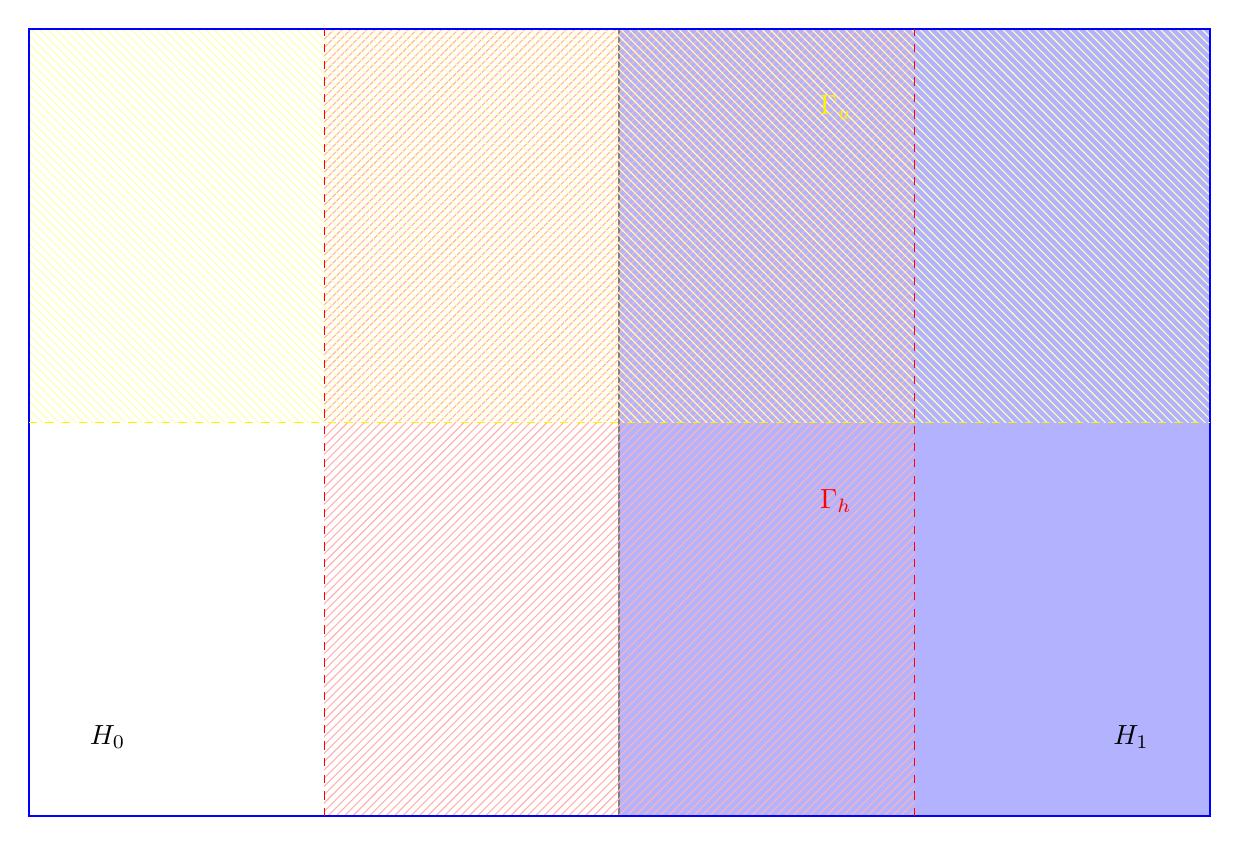
\begin{tikzpicture}
\fill[color=blue!30] (7.5,0) rectangle (15,10);
\draw[gray, thick] (7.5,0) -- (7.5,10);
\fill[pattern=north east lines, pattern color=red!30] (3.75,0) rectangle (11.25,10);
\fill[pattern=north west lines, pattern color=yellow!30] (0,5) rectangle (15,10);
\draw[blue, thick] (0,0) rectangle (15,10);
\draw[dashed, color=yellow] (0,5) -- (15,5);
\draw[dashed, color=red] (3.75,0) -- (3.75,10);
\draw[dashed, color=red] (11.25,0) -- (11.25,10);
\node[] at (1,1) {$H_0$};
\node[] at (14,1) {$H_1$};
\node[color=red] at (10.25,4) {$\Gamma_h$};
\node[color=yellow] at (10.25,9) {$\Gamma_u$};
\end{tikzpicture}
\caption{The cylinder $\Gamma_L$.}
\label{fig:setup}
\end{figure}

We also consider the plane $\Z^2$. In this setting, there are no edge states, and so the associated ``bulk" Hamiltonian $H_B$ is assumed to have a \textit{gapped} spectrum, in the sense that

\begin{assumption}
\[\emph{Spec}(H_B) = \mathcal{S}_{-} \cup \mathcal{S}_{+},\]
where $\inf\mathcal{S}_{+} - \sup \mathcal{S}_{-} \geq \gamma$ uniformly in $L$ and $\mu$ for some $\gamma > 0$. 
\label{ass:gap}
\end{assumption}

In the case of the cylinder, this effect does not necessarily occur due to the presence of the edge. 
We also assume that the Hamiltonian is \emph{charge-conserving}.

\begin{assumption}
$[H_\mu, Q] = 0$, where $Q$ is the total charge in $\Gamma_L$.
\label{ass:charge}
\end{assumption}

Let $P_B$ be the ground state projection of $H_B$ (the system without an edge), and let $P$ be the ground state projection of $H$ (the system with an edge). We assume that states far from the edge are essentially bulk states, up to tails that vanish quickly in $L$.

\begin{assumption}
Define the \emph{edge region }

\[\Gamma_E = [L/2-k,L/2+k]\times [0,L] \cup [L-k,k]\times [0,L].\]

for some $k>0$. For any operator $A$ supported on $\Gamma_E^\mathsf{c}$,

\[\emph{Tr}(PA) = \emph{Tr}(P_BA) + \mathcal{O}(L^{-\infty}).\]

The $A$ on the right hand side is understood to be the extension by zeroes of $A$ to the plane $\Z^2$.
\label{ass:bulk}
\end{assumption}

The idea is that observables localized far away from the edge are not affected by the edge of the system. We similarly define the \emph{bulk region}

\[\Gamma_B = [3L/4-k, 3L/4+k] \times [0,L],\]

and the \emph{middle region}

\[\Gamma_m = [L/2,L]\cup[0,L] \setminus (\Gamma_E \cup \Gamma_B).\]

The three regions are depicted in figure \ref{fig:regions}.

\newpage
\begin{figure}[h!]
\centering
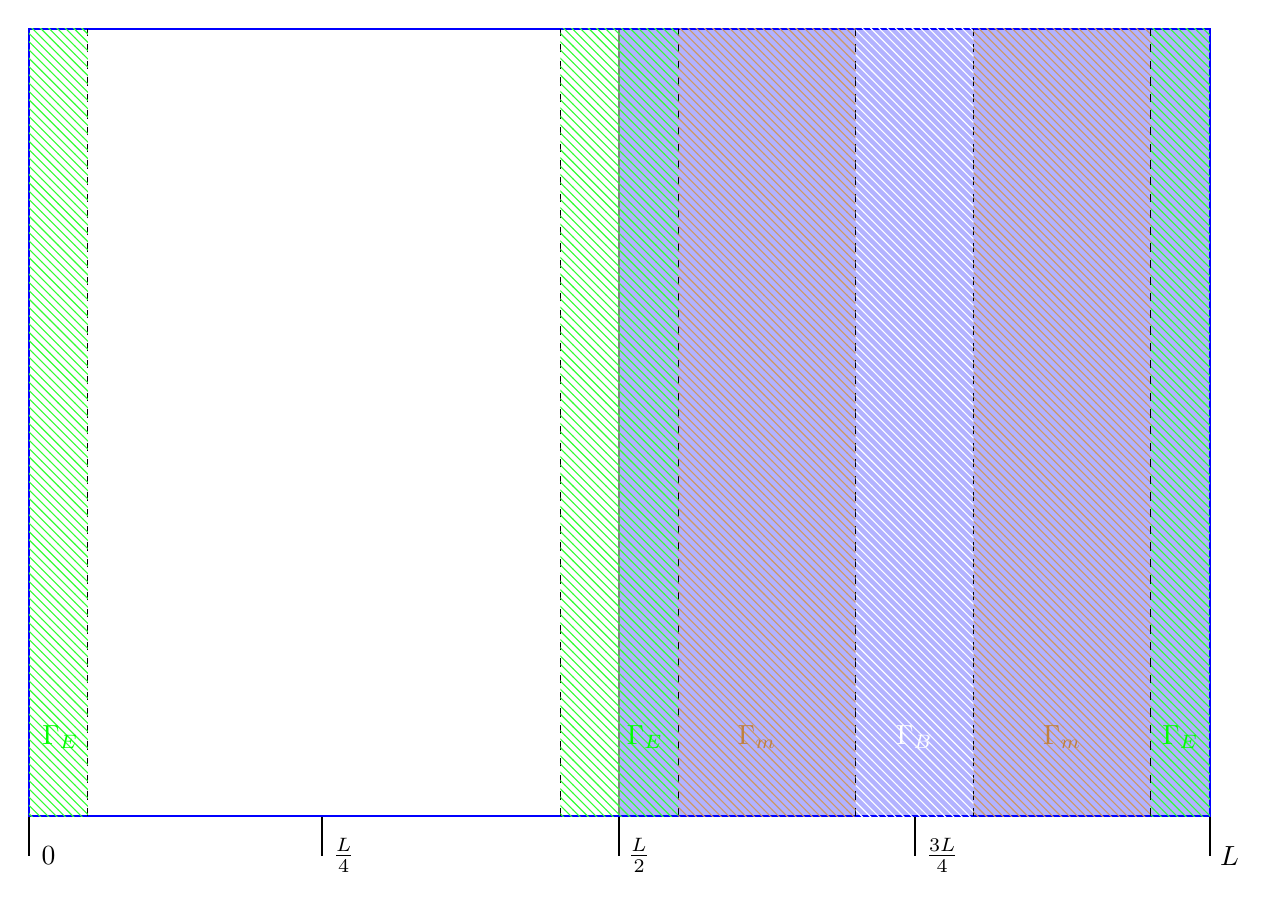
\begin{tikzpicture}
\fill[color=blue!30] (7.5,0) rectangle (15,10);
\draw[gray, thick] (7.5,0) -- (7.5,10);

\draw[black,thick] (0,-0.5) -- (0,0);
\node[] at (0.25,-0.5) {$0$};
\draw[black,thick] (3.725,-0.5) -- (3.725,0);
\node[] at (4,-0.5) {$\frac{L}{4}$};
\draw[black,thick] (7.5,-0.5) -- (7.5,0);
\node[] at (7.75,-0.5) {$\frac{L}{2}$};
\draw[black,thick] (11.25,-0.5) -- (11.25,0);
\node[] at (11.6,-0.5) {$\frac{3L}{4}$};
\draw[black,thick] (15,-0.5) -- (15,0);
\node[] at (15.25,-0.5) {$L$};

%\fill[pattern=north east lines, pattern color=red!30] (3.75,0) rectangle (11.25,10);
%\fill[pattern=north west lines, pattern color=yellow!30] (0,5) rectangle (15,10);
\draw[blue, thick] (0,0) rectangle (15,10);
%\draw[dashed, color=yellow] (0,5) -- (15,5);
%\draw[dashed, color=red] (3.75,0) -- (3.75,10);
%\draw[dashed, color=red] (11.25,0) -- (11.25,10);
%\node[] at (1,1) {$H_0$};
%\node[] at (14,1) {$H_1$};
%\node[color=red] at (10.25,4) {$\Gamma_h$};
%\node[color=yellow] at (10.25,9) {$\Gamma_u$};

\draw[dashed, color=black] (6.75,0) -- (6.75,10);
\draw[dashed, color=black] (8.25,0) -- (8.25,10);
\fill[pattern=north west lines, pattern color=green!80] (6.75,0) rectangle (8.25,10);
\node[color=green] at (7.825,1) {$\Gamma_E$};

%\draw[dashed, color=brown] (8.25,0) -- (8.25,10);
%\draw[dashed, color=brown] (10.5,0) -- (10.5,10);
\fill[pattern=north west lines, pattern color=brown!80] (8.25,0) rectangle (10.5,10);
\node[color=brown] at (9.25,1) {$\Gamma_m$};

\draw[dashed, color=black] (10.5,0) -- (10.5,10);
\draw[dashed, color=black] (12,0) -- (12,10);
\fill[pattern=north west lines, pattern color=white!80] (10.5,0) rectangle (12,10);
\node[color=white] at (11.25,1) {$\Gamma_B$};

%\draw[dashed, color=brown] (12,0) -- (12,10);
%\draw[dashed, color=brown] (14.25,0) -- (14.25,10);
\fill[pattern=north west lines, pattern color=brown!80] (12,0) rectangle (14.25,10);
\node[color=brown] at (13.125,1) {$\Gamma_m$};

\draw[dashed, color=black] (14.25,0) -- (14.25,10);
\fill[pattern=north west lines, pattern color=green!80] (14.25,0) rectangle (15,10);
\node[color=green] at (14.625,1) {$\Gamma_E$};

\draw[dashed, color=black] (0.75,0) -- (0.75,10);
\fill[pattern=north west lines, pattern color=green!80] (0,0) rectangle (0.75,10);
\node[color=green] at (0.4,1) {$\Gamma_E$};
\end{tikzpicture}
\caption{The regions $\Gamma_E$, $\Gamma_B$, and $\Gamma_m$.}
\label{fig:regions}
\end{figure}




\subsection{Equality of Bulk and Edge Currents}

\subsubsection{Cylinder Geometry}

Let $P_\mu$ be the (possibly degenerate) ground state projection of $H_\mu$. Let $Q_u = \sum_{x \in \Gamma_u} a_x^* a_x$ be the charge in the upper half of the cylinder $\Gamma_u = [0,L] \times [L/2,L]$ (the yellow region in Figure \ref{fig:setup}), and define current operator 

\[J = i[H_\mu,Q_u],\]

which measures the current across the fiducial line $y=L/2$. Charge conservation~\ref{ass:charge} implies that this current operator is supported along a strip of width $2R$ centred on the fiducial line $y=L/2$. Indeed, if we inspect a local interaction $\Phi(X)$ of range $R$ with support $(\Gamma_u)_R$, where $(X)_\alpha$ is the $\alpha$-shrinking of the set $X$, then clearly $\Phi(X)$ commutes with the charge outside $\Gamma_u$, so that $[\Phi(X), Q_u] = [\Phi(X), Q]$, which vanishes by the charge conservation assumption~\ref{ass:charge}. Similarly, if $\Phi(X)$ is supported in $((\Gamma_u)^\mathsf{c})_R$, then $[\Phi(X), Q_u] = [\Phi(X), Q] = 0$. It follows that for an interaction $\Phi(X)$ with range $R$ and arbitrary support, $[\Phi(X), Q_u]$ must be supported on a set which is contained in (or equal to) the strip $[L/2, L] \times [L/2-R, L/2+R]$. There $[H_\mu,Q_u]$ must be supported there as well, since $H_\mu$ is a sum of such local interactions. 

From this point, we drop the subscript $\mu$ wherever it is not needed for context.

% In the case of a unique ground state $\Omega$, the total change in charge in $\Gamma_h$ after threading one quantum of flux is given by the fundamental theorem of calculus,

%\[ \int_{t:\Phi = 0}^{t:\Phi=2\pi} i[H, Q_u] dt' = \langle \Omega, (U^* Q_h U - Q_h) \Omega \rangle\]

\begin{lemma}
The ground state expectation of the current $J$ is zero.
\label{lemma:J=0}
\end{lemma}

\begin{proof}
Assuming linearity and cyclicity of the trace hold, the proof is trivial, 

\[\begin{aligned}
\Tr(P J) = i\Tr(P [H,Q_u]) = i\Tr([P,H]Q_u) = 0.
\end{aligned}\]

In order for this calculation to hold, we need to prove that

\begin{enumerate}
\item $P H Q_u$ and $P Q_u H$ are separately trace-class to apply linearity of the trace, and 
\item $\norm{H}<\infty$ and $P Q_u \in \mathcal{J}_1$ to apply cyclicity of the trace. 
\end{enumerate}

The latter implies the former by the bound $\norm{AB}_1 \leq \norm{A}_1\norm{B}$.  To prove (2), fix a finite $L$. The Hamiltonian is bounded since it is a finite sum of at most $\mathcal{P}(\Gamma_L)$ local interactions $\Phi(X)$, each of which is uniformly bounded by assumption, along with the $\mu Q_h$ term. But the number operator for the entire space is bounded by $\norm{Q} \leq NL^2$, where $N$ is the uniform bound on the dimension of each Hilbert space. This shows that both $Q_u$ and $Q_h$ are bounded in operator norm. Finally, $\norm{P}_1\leq CL^2$ because the projection is finite-rank, since the dimension of each site is bounded. Therefore $P Q_u \in \mathcal{J}_1$.

%\[\begin{aligned}
%\norm{P_\mu H_\mu}_1 &= \norm{P_\mu\sum_{X\in \Gamma_L}\Phi(X) + P_\mu \mu Q_h}_1\\
%&\leq \sum_{X\in\Gamma_L} \norm{P_\mu \Phi(X)}_1 + \mu\norm{P_\mu Q_h}_1\\
%&\leq \norm{P_\mu}_1 \sum_{X\in\Gamma_L} \norm{\Phi(X)}+ \mu \norm{P_\mu}_1\norm{Q_h}\\
%\end{aligned}\]
\end{proof}

Next, we define a family of operators indexed by $\mu$ called \emph{Hastings operators},

\[K_\mu = \mathcal{I}_{\mu}(\dot{H}_\mu),\]

where 

\[\mathcal{I}_{\mu} (A) = \int_\R W(t) e^{itH_\mu} A e^{-itH_\mu}dt.\]

Here, $W:\R\to\R$ is a function satisfying (need to add). More explicitly, in our setting we see that 

\[K_\mu = \mathcal{I}_\mu(Q_h).\]

 %As a shorthand, we use the notation $\dot{A}_{\mu_0}= (\frac{d}{d\mu}A_\mu)|_{\mu=\mu_0}$. 

We present two important properties of the map $\mathcal{I}_\mu:\mathcal{U}_L\to\mathcal{U}_L$ in the following lemmas, and leave their proofs to the appendix (need to add). 

First, recall a definition from the non-interacting setting: an \emph{off-diagonal} operator is an operator $A$ such that $A = \overline{A} := P_\mu AP_\mu^\perp + P_\mu^\perp AP_\mu$, where $P_\mu^\perp = \mathbb{I} - P_\mu$ is the projection onto the excited states above the gap.

\begin{lemma}
\begin{enumerate}
\item For any off-diagonal operator $A=\overline{A}$, $\mathcal{I}_\mu(\cdot)$ and $[H_\mu, \cdot]$ act as inverses of each other, up to a factor of $i$:

\[\mathcal{I}_\mu\left([H_\mu, A]\right) = [H_\mu, \mathcal{I}_\mu(A)] = iA.\]

\item For any (not necessarily off-diagonal) operator $A$, 

\[[\mathcal{I}_\mu([H_\mu, A]),P_\mu] = i[A,P_\mu].\]
\end{enumerate}
\label{lemma:inverseofH}
\end{lemma}

%It is easy to verify that any operator $A$ behaves as an off-diagonal operator when taking a commutator with $P$, in the sense that

%\[[\overline{A}, P] = [A,P].\]

%Combining this fact with Lemma \ref{lemma:inverseofH}, it follows that for any (not necessarily off-diagonal) operator $A$, 

%\[[\mathcal{I}_\mu([H_\mu, A]),P_\mu] = i[A,P_\mu].\]

Another important property of the map $\mathcal{I}_\mu$ is that it preserves locality.

\begin{lemma}
$\mathcal{I}_\mu$ is local in the sense that for any $A \in \mathcal{U}_X$, 

\[\norm{\mathcal{I}(A)_{(X^r)^\mathsf{c}}} \leq \norm{A} |X| \mathcal{O}(r^{-\infty})\]

where $X^r = X \cup \{ x : d(x,X) \leq r\}$ is the $r$-fattening of $X$.
\label{lemma:local}
\end{lemma}

\begin{proposition}
The operator $K_\mu$ is the \emph{generator of parallel transport}, satisfying
\[\dot{P}_\mu = i[K_\mu,P_\mu]\]
for all $\mu$.
\label{prop:generatorparalleltransport}
\end{proposition}
\begin{proof}
First, we show that $\dot{P}$ is off-diagonal. Taking the derivative on both sides of $P^2=P$, we see that $\dot{P} P + P \dot{P} = \dot{P}$. Acting on the left and right with $P$ on both sides of this equation gives 

\[P\dot{P}P + P\dot{P}P = P\dot{P}P,\]

which implies that $P\dot{P}P = 0$. Thus 

\[\begin{aligned}
\overline{\partial_\mu P} &= P\dot{P}(1-P) + (1-P)\dot{P}P\\
&= P\dot{P} - P\dot{P}P + \dot{P}P - P\dot{P}P\\
&= P\dot{P} + \dot{P}P\\
&= \partial_\mu (P^2)\\
&= \partial_\mu P,
\end{aligned}\]

as claimed. By the product rule and the fact that $H$ and $P$ commute, 

\[ [\dot{H}, P] = -[H, \dot{P}]. \]

It therefore follows from Lemma~\ref{lemma:inverseofH} that 

\[\begin{aligned}
\dot{P} &= -i \mathcal{I}_\mu([H, \dot{P}]) = i\mathcal{I}([\dot{H}, P]) = i[\mathcal{I}(\dot{H}), P] = i[K, P].
\end{aligned}\]
\end{proof}

Increasing the electric potential by a small amount $d\mu Q_h$ and expanding to linear order, the change in ground state current is given by

\[\Tr(P_{\mu+d\mu}J) - \Tr(P_\mu J) = \kappa d\mu + \mathcal{O}(d\mu^2).\]

Dividing by $d\mu$ and taking a limit, we see that the linear response coefficient is given by

\[\sigma(\mu) = \Tr\left(\dot{P}_\mu J\right).\]

The \emph{Hall conductivity} of the system on a subset $V \subseteq \Gamma_L$ is defined to be $\sigma_V := \Tr\left(\dot{P} J_V\right)$, where $J_V$ is the restriction of $J$ to $V$. 

\begin{proposition}
The Hall conductivity is independent of the driving strength $\mu$.
\label{prop:independent}
\end{proposition}
\begin{proof}

%Since $\dot{H}_\mu=Q_h$, we see that $\dot{J} = 0$. Thus $\frac{d}{d\mu} \Tr(P_\mu J) = \sigma(\mu)$. 

For any $\mu_1$ and $\mu_2$,

%\[\begin{aligned}
%\sigma(\mu_1) - \sigma(\mu_2) &= \frac{d}{d\mu} \Tr\left( P_{\mu_1} i[H_{\mu_1}, Q_u] - P_{\mu_2}i[H_{\mu_2},Q_u]\right)\\
%&= i\frac{d}{d\mu} \Tr\left(\left([P_{\mu_1}, H_{\mu_1}] - [P_{\mu_2}, H_{\mu_2}]\right)Q_u\right)\\
%&= 0
%\end{aligned}\]
%^Doesn't work because otherwise \sigma=0 always.


\[\begin{aligned}
\sigma(\mu_1) - \sigma(\mu_2) &= \Tr\left( \dot{P}_{\mu_1} i[H_{\mu_1}, Q_u] - \dot{P}_{\mu_2}i[H_{\mu_2},Q_u]\right)\\
&= i\Tr\left(\left([\dot{P}_{\mu_1}, H_{\mu_1}] - [\dot{P}_{\mu_2}, H_{\mu_2}]\right)Q_u\right)\\
&= - i\Tr\left(\left([\dot{H}_{\mu_1}, P_{\mu_1}] - [\dot{H}_{\mu_2}, P_{\mu_2}]\right)Q_u\right)\\
&= i\Tr\left( [Q_h, P_{\mu_1} - P_{\mu_2}]Q_u \right)\\
&= i\Tr\left( [Q_u,Q_h]( P_{\mu_1} - P_{\mu_2})\right)\\
&= 0,
\end{aligned}\]
% Would need to bound \norm{\dot{P}}_1 to do this ^.

since $H$ and $P$ commute. Note that $\norm{\dot{P}}_1<\infty$ since we are working in a finite-dimensional space. The proof of Lemma \ref{lemma:J=0} provides the other necessary bounds to invoke linearity and cyclicity of the trace to shift the commutator in the second line and second-last line.
\end{proof}

This indicates that the Hall conductivity is independent of $\mu$ as one would expect physically. We simply write $\sigma=\sigma(\mu)$ from this point, in accordance with proposition \ref{prop:independent}. 

The following is the main result:

\begin{theorem}
Let $V \subseteq \Gamma_m$ be a set contained within the strip in between the edge region $\Gamma_E$ and the bulk region $\Gamma_B$ (see Figure \ref{fig:regions}), and define the distance

\[r = \emph{dist}(V, \Gamma_E \cup \Gamma_B)\]

from $V$ to the bulk and edge regions. The Hall conductivity in this regions vanishes in the sense that

\[\sigma_V = \mathcal{O}(r^{-\infty}) + \mathcal{O}(L^{-\infty}).\]

\end{theorem}

\begin{proof}
By Proposition~\ref{prop:generatorparalleltransport}, the bulk Hall conductivity can also be written by the formula 

\[\sigma_V^B = \Tr\left(i[K,P_B]J_V^B\right) = \Tr\left(i[\mathcal{I}(Q_h), P_B]J_V^B\right),\]

where $J_V^B = i[H_B, Q_u]|_V$ is the current in the region $V$ arising from the bulk Hamiltonian. From commutativity of $P_B$ and $H_B$ along with cyclicity of the trace, we compute

\[\begin{aligned}
\sigma_V^B &= \Tr\left(i\int_\R W(t) e^{itH_B} [Q_h,P_B] e^{-itH_B}dt J_V^B \right)\\
&= \int_\R W(t) \Tr\left(i[Q_h,P_B] e^{-itH_B}J_V^Be^{itH_B}\right)dt\\
&= -\int_\R W(t) \Tr\left(i[Q_h,P_B] e^{itH_B}J_V^Be^{-itH_B}\right)dt\\
&=- \Tr\left(i[Q_h,P_B]\mathcal{I}(J_V^B)\right),
\end{aligned}\]

since $W(t)$ is odd. By part (2) of Lemma \ref{lemma:inverseofH}, we have $i[Q_h,P_B] = [\mathcal{I}([H_B,Q_h]),P_B]$. Therefore

\[\begin{aligned}
\sigma_V^B &=-\Tr([\mathcal{I}([H_B,Q_h]), P_B]\mathcal{I}(J_V^B))\\
&= \Tr\left( P_B[\mathcal{I}([H_B,Q_h]), \mathcal{I}(J_V^B)]\right).
\end{aligned}\]

Now, $[H_B, Q_h]$ is a local operator supported on $\Gamma_B$, while $J_V^B$ is a local operator supported on $V \cap \Gamma_B = \varnothing$. Since $\mathcal{I}$ preserves locality up to tails, in the sense that $\norm{\mathcal{I}(A)_{(S^r)^\mathsf{c}}} \leq \norm{A} |S| \mathcal{O}(r^{-\infty})$ for any operator $A$ supported in $S$ (Lemma~\ref{lemma:local}), it follows that the commutator can be written

\[[\mathcal{I}([H_B,Q_h])|_{\Gamma_B} + \mathcal{O}(r^{-\infty}) A_1, \mathcal{I}(J_V^B)|_V + \mathcal{O}(r^{-\infty}) A_2] = C\mathcal{O}(r^{-\infty}),\]

for some operators $A_1$ and $A_2$ supported on $\Gamma_B^\mathsf{c}$ and $V^\mathsf{c}$, respectively. This fact applies to the bulk setting with $H_B$ and $P_B$. To extend this to the setting with an edge, it is enough to use Assumption~\ref{ass:bulk} to conclude the same result, except with equality up to $\mathcal{O}(L^{-\infty})$, i.e.

\[\sigma_V = \Tr\left(\dot{P}J_V\right) = \Tr\left(\dot{P}(J_V^B + \mathcal{O}(L^{-\infty}))\right) = \sigma_V^B + \mathcal{O}(L^{-\infty}) = \mathcal{O}(r^{-\infty}) + \mathcal{O}(L^{-\infty}).\]

\end{proof}


The intuitive picture from the previous result is that, in the bulk region, the Hall conductivity is essentially only nonzero along  the bulk strip $\Gamma_B$. Since the ground state expectation of the current is zero (by lemma~\ref{lemma:J=0}), it must be that there is an equal current flowing along the edge strip $\Gamma_E$, but in the opposite direction.

\subsubsection{Torus Geometry}

Our goal is to show the same result on the discrete torus $\mathbb{T}_L := \Z_L \times \Z_L$. We define the same regions $\Gamma_u$ and $\Gamma_h$, and the same current operator $J_u = i[H(\mu), Q_u]$. This time, however, Lemma~\ref{lemma:J=0} does not apply. Intuitively, it does not apply because electrons can now flow through both the bottom and the top of the region $\Gamma_u$, rather than just the bottom. Mathematically, the lemma fails because our definition of the current is slightly changed.

We use charge conservation and the fact that $H$ is finite range to split the current $J_u$ into two components, $J_u = i[H_-, Q_u] + i[H_+, Q_u] = J_- - J_+$, supported on strips of width $2R$ at $y=L/2$ and $y=L$, respectively. We then define the current operator to be $J=J_-$, which is the current on the lower strip. This is the mathematical reason that the proof in Lemma~\ref{lemma:J=0} fails on the torus; we have replaced $H$ by $H_-$, which may no longer commute with $P$. We instead proceed by a different approach. We will need a few auxiliary results first.

\begin{lemma}
$K_\pm$ is supported on $\partial_\pm$ up to tails.
\label{SupportOfK}
\end{lemma}
\begin{proof}

\end{proof}

\begin{proposition}
The operator $Q_h-K$ leaves the ground state space invariant, i.e. $[Q_h-K, P] = 0$.
\end{proposition}
\begin{proof}

\end{proof}


\begin{lemma}
Show that $\emph{Tr}(A,[Q_h,P])=0$ for all $A \in \mathcal{U}_{\text{edge}}$. This shows that $Q_h$ commutes with $P$ ``along the edge".
\label{lemma:[Q,P]=0}
\end{lemma}
\begin{proof}

Let $A \in \mathcal{U}_{\text{edge}}$. Since $H$ is charge conserving, we may choose a simultaneous eigenbasis of $H$ and the total charge $Q$, in which case $P$ and $Q$ commute. It follows that

\[\begin{aligned}
\Tr(A[Q_h, P]) = \Tr([A, Q_h] P) = \Tr([A, Q]P) = \Tr(A[Q,P]) = 0.
\end{aligned}\]



%\[\begin{aligned}
%\Tr(A [Q_h, P]) &= \Tr([A, Q_h]P)\\
%&= \Tr([P,A]Q_h)\\
%&= \sum_{x \in \Gamma_h} \Tr([P, A] c_x^*c_x)\\
%&= \sum_{x \in \Gamma_h} \Tr\left(\bigotimes_{y \in \text{supp}([P, A])} \left[P, A\right]_y c_x^*c_x\right)\\
%&= \sum_{x \in \Gamma_h} \Tr\left(\bigotimes_{y \in \text{supp}([P, A])} \left[P_y, A_y\right] c_x^*c_x\right)\\
%&= \sum_{x \in \Gamma_h} \prod_{y \in \text{supp}([P, A])} \Tr([P_y, A_y] c_x^*c_x)
%\end{aligned}\]

%The support of $[P, A]$ is the edge, so

%\[\begin{aligned}
%\Tr(A [Q_h, P]) &= \sum_{x \in \Gamma_h} \prod_{y \in \text{edge}} \Tr([P_y, A_y] c_x^*c_x)\\
%&= \sum_{x \in \Gamma_h} \prod_{y \in \text{edge}} \Tr((\mathbb{I}\otimes\ldots\otimes\mathbb{I}\otimes [P_y, A_y] \otimes\mathbb{I}\ldots\otimes\mathbb{I}) (\mathbb{I}\otimes \ldots \otimes\mathbb{I} \otimes c^*_xc_x \otimes \mathbb{I} \ldots\otimes\mathbb{I}))\\
%&= \sum_{x \in \Gamma_h} \prod_{y \in \text{edge}} \Tr(\mathbb{I}\otimes\ldots\otimes\mathbb{I}\otimes c_x^*c_x \otimes \mathbb{I} \otimes \ldots \otimes\mathbb{I} \otimes [P_y, A_y] \otimes\mathbb{I}\ldots)\\
%&= \sum_{x \in \Gamma_h} \prod_{y \in \text{edge}, \; y\neq x} \Tr(c_x^*c_x)\Tr([P_y, A_y]) + \sum_{x \in \Gamma_h \cap \text{edge}} \Tr(c_x^*c_x [P_x, A_x]).\\
%\end{aligned}\]

%Since the trace of any commutator is zero, the terms in the first sum vanish. Since $\Gamma_h \cap \text{edge} =\text{edge}$, we are left with

%\[\Tr(A[Q_h, P]) = \sum_{x \in \text{edge}} \Tr(c_x^*c_x[P_x, A_x]) = \sum_{x \in \text{edge}} \Tr(P_x[A_x, c_x^*c_x]).\]

%For any particular $x\in \text{edge}$, write $P_x = \sum_n |\psi_n \rangle \langle \psi_n |$, where the sum is over ground states, and 

%\[\langle \psi | [P_y, A_y]|\psi\rangle = \sum_n \langle \psi | \psi_n \rangle \langle\psi_n | A |\psi\rangle - \sum_n \langle \psi | A |\psi_n\rangle\langle\psi_n | \psi\rangle \]

%Want to show:

%\[\Tr([P_y, A_y]) = \ldots = 0\]

\end{proof}

Finally, we will prove that in the bulk system with Hamiltonian $H_B(\mu)$, the ground state expectation of the current vanishes faster than any power as $L \to \infty$.

\begin{lemma}
The ground state expectation of the current $J_B := i[(H_B)_-, Q_h]$ (of the system without an edge) is $\emph{Tr}(P_BJ_B)=\mathcal{O}(L^{-\infty})$.
\label{J=0Bulk}
\end{lemma}
\begin{proof}
First, $K = \mathcal{I}(i[H_B, Q])$ splits into $K = K_- - K_+$, with the support of $K_\pm$ contained in $\partial_\pm$ up to tails:

\[[K_\pm, A_X] = \mathcal{O}(p^{-\infty}),\]

for every $A_X \in \mathcal{U}_X$ such that $\norm{A_X}=1$, and where $p = \text{dist}(X, \partial_\pm)$ (need to add). Using the fact that $K_\pm$ is supported in $\partial_\pm$ up to tails (Lemma~\ref{SupportOfK}), we see that 

\[i[H_B, K_-] = i[(H_B)_-, K_-] + \mathcal{O}(L^{-\infty}),\]

and similarly $i[(H_B)_-, K_+] = \mathcal{O}(L^{-\infty})$. Putting these facts together, it follows that the current can be rewritten as 

\[\begin{aligned} 
J _B&= i[H_B, Q_h + K_- - K_- + K_+] + \mathcal{O}(L^{-\infty})\\
&= i[H_B, K_-] + i[(H_B)_-, Q_h - K_- + K_+)] + \mathcal{O}(L^{-\infty}).
\end{aligned}\]

From here, we use the fact that $H_B$ and $Q_h-K_-+K_+$ both commute with $P_B$ to write

\[P_BJ_BP_B = i[H_B, P_BK_-P_B] + i[P_B(H_B)_-P_B, Q_h - K_- + K_+)] + P_B\mathcal{O}(L^{-\infty})P_B.\]

Since the trace of any commutator is zero, 

\[\Tr(P_BJ_B) = \Tr(P_BJ_BP_B) = \mathcal{O}(L^{-\infty}).\]

\end{proof}

Using this, we can show a simple proof of the analogue of Lemma~\ref{lemma:J=0} on the torus, in the case of non-interacting systems.

\begin{proposition}
Let $H = \sum_{x \in \mathbb{T}} h_x$ be a non-interacting Hamiltonian, i.e. a sum of single site Hamiltonians $h_x$. The ground state expectation of the current $J=i[H_-, Q_h]$ (of the system with an edge) is $\emph{Tr}(PJ)=\mathcal{O}(L^{-\infty})$.
\label{prop:J=0Torus}
\end{proposition}

\begin{proof}

Since $H$ is a sum of single site Hamiltonians, we can split $H_-$ into the restrictions $H_- = (H_-)_\text{edge} + (H_-)_\text{bulk}$, with no fear of any terms which are in both the edge region and the bulk region. By Assumption~\ref{ass:bulk},

\[\begin{aligned}
\Tr(PJ) &= \Tr(Pi[H_-, Q_h])\\
&= i\Tr([H_-, Q_h]P)\\
&= i\Tr((H_-)_\text{edge} [Q_h, P]) + i \Tr((H_-)_\text{bulk} [Q_h, P])\\
&= i\Tr((H_-)_\text{edge} [Q_h, P]) + i \Tr((H_-)_\text{bulk} [Q_h, (P)_\text{bulk}])\\
&= i\Tr((H_-)_\text{edge} [Q_h, P]) + i \Tr((H_B)_-[Q_h, P_B]) + \mathcal{O}(L^{-\infty})\\
&= i\Tr((H_-)_\text{edge} [Q_h, P]) + \Tr(i[(H_B)_-, Q_h]P_B) + \mathcal{O}(L^{-\infty}).
\end{aligned}\]

By Lemma~\ref{lemma:[Q,P]=0}, the first term is zero. By Lemma~\ref{J=0Bulk}, the second term is $\mathcal{O}(L^{-\infty})$. 
\end{proof}

\newpage
\appendix

\section{Properties of $\mathcal{I}_\mu$}

\begin{proof}
(Of Lemma~\ref{lemma:inverseofH}). Let $\widehat{W}(\xi) = \frac{1}{\sqrt{2\pi}}\int_\R W(t) e^{-2\pi i t \xi} dt$ be the Fourier transform of $W$. One can show that for $|\xi|\geq \gamma$, $\widehat{W}(\xi) = \frac{1}{\sqrt{2\pi}i \xi}$ (need to add). Let $A$ be an observable. First, we show that $\mathcal{I}([H,PAP^\perp]) = iPAP^\perp$. 

Decomposing 

\[\begin{aligned}
e^{itH}P &= \sum_{j=0}^\infty \frac{(itH)^j}{j!} P \\
&= \sum_{j =0}^\infty \frac{(it)^j}{j!} \left(\sum_n E_n^j P_n\right)P \\
&= \sum_{j=0}^\infty \frac{(it)^j}{j!} \sum_{n : E_n=0} E_n^j P_n \\
&= \sum_{n : E_n=0} e^{itE_n}P_n,
\end{aligned}\]

and similarly 

\[P^\perp e^{-itH}= \sum_{m:E_m \geq \gamma}P_m e^{-itE_m},\]

we see that

\[\begin{aligned}
\mathcal{I}([H,PAP^\perp]) &= \mathcal{I}(P[H,A]P^\perp) \\
&= \int_\R W(t)e^{itH}P[H,A]P^\perp e^{-itH}dt \\
&= \int_\R W(t) \sum_{n : E_n=0} e^{itE_n}P_n [H,A] \sum_{m:E_m \geq \gamma} P_m e^{-itE_m} dt\\
&= \sum_{n : E_n=0} \sum_{m:E_m \geq \gamma} \int_\R W(t) e^{itE_n} P_n A (E_n-E_m) P_m e^{-itE_m}dt\\
&= \sum_{n : E_n=0} \sum_{m:E_m \geq \gamma} P_n A P_m (E_n-E_m) \int_\R W(t) e^{-it(E_m - E_n)} dt\\
&= \sum_{n : E_n=0} \sum_{m:E_m \geq \gamma} P_n A P_m (E_n-E_m) \sqrt{2\pi} \widehat{W}(E_m-E_n) \\
&= i\sum_{n : E_n=0} \sum_{m:E_m \geq \gamma} P_n A P_m\\
&= iPAP^\perp.
\end{aligned}\]

(need to check the $2\pi$ factor)

By the same argument, $\mathcal{I}([H,P^\perp AP]) = iP^\perp AP$ as well, and so $\mathcal{I}([H,\overline{A}]) = i\overline{A}$.
\end{proof}

\begin{proof}

(Of Lemma~\ref{lemma:local}). We break the integral into two parts,

\[\norm{\mathcal{I}(A)} \leq \bigg\lVert\int_{-T}^T W(t) e^{itH}Ae^{-itH}dt \bigg\rVert + \bigg\lVert \int_{\R\setminus [-T,T]} W(t) e^{itH}Ae^{-itH}dt\bigg\rVert.\]

The first term can be estimated using the Lieb-Robinson bound found in Appendix~\ref{sec:L-R}.

\end{proof}

\section{Lieb-Robinson Bound}
\label{sec:L-R}

Let $N$ be a uniform upper bound for the dimensions of the Hilbert spaces at each site, i.e. $\text{dim}(\mathcal{H}_x) \leq N$ for all sites $x$.

The following is a version of the Lieb-Robinson. For any operators $A \in \mathcal{U}_X$ and $B \in \mathcal{U}_Y$ having disjoint supports $X\cap Y = \varnothing$, 

\[\norm{ [e^{itH}Ae^{-itH}, B] } \leq  C \norm{A}\norm{B} |X| |Y| N^{2|X|} e^{2t\norm{\Phi}_\lambda - \lambda d(X, Y)}.\]

\section{Gr\"{o}nwall's Inequality and Uniqueness}

\begin{theorem}
(Gr\"{o}nwall's Inequality). Let $\alpha : I \to (0,\infty)$ be positive and continuous on $I^o$ for some interval of the form $[a,b)$, $[a,b]$, or $[a,\infty)$. Suppose $u : \mathbb{R} \to \mathcal{U}$ is a Banach-valued, differentiable function. If $\norm{u'(t)} \leq \alpha(t)\norm{u(t)}$ for all $t\in I$, then 
\[\norm{u(t)} \leq \norm{u(a)} e^{\int_a^t \alpha(s)ds} \quad \forall t\in I\]
\end{theorem}
\label{thm:gronwallinequality}
\begin{proof}
Let $f(t) = e^{\int_a^t \alpha(s)ds}$, which is nonzero, has initial value $f(a)=1$, and has derivative $f'(t) = \alpha(t) f(t)$. Then by the quotient rule,
\[\left(\frac{\norm{u(t)}}{f(t)}\right)' = \frac{\norm{u'(t)}f(t) - \norm{u(t)}\alpha(t)f(t)}{f(t)^2} \leq 0,\]
where the inequality follows from the assumption $\norm{u'(t)} \leq \norm{\alpha(t)u(t)}$. Thus $\frac{\norm{u(t)}}{f(t)}$ is decreasing, so that 
\[\frac{\norm{u(t)}}{f(t)} \leq \frac{\norm{u(a)}}{f(a)} = \norm{u(a)},\]
which is the desired inequality.
\end{proof}

\begin{theorem}
(ODE Uniqueness). Let $F:\mathcal{U}\to\mathcal{U}$ be Lipschitz and consider the differential equaton $u'(t)=F(u(t))$ with initial condition $u(a) = u_a$ for some function $u:I\to\mathcal{U}$, where $I = [a,b]$, or $[a,b)$, or $[a,\infty)$. Solutions to this equation are unique.
\end{theorem}
\label{thm:gronwalluniqueness}
\begin{proof}
Suppose there are two solutions $u(t)$ and $v(t)$, and let $g(t) = \norm{u(t)-v(t)}^2$. By assumption, there exists a constant $L_F$ such that $\norm{F(u(t))-F(v(t))} \leq L_F \norm{u(t)-v(t)}$, so that
\[\begin{aligned}
g'(t) &= 2\norm{u(t)-v(t)}\norm{u'(t)-v'(t)}\\
&=2\norm{u(t)-v(t)}\norm{F(u(t))-F(v(t))}\\
&\leq 2L_F\norm{u(t)-v(t)}^2\\
&= 2L_F g(t).
\end{aligned}\]
Notice that $\alpha := 2L_F$ is a positive continuous function, so we may apply Gr\"{o}nwall's inequality to $g(t)$ to conclude
\[g(t) \leq g(a)e^{2L_f(t-a)} = 0,\]
since $g(a)=0$.
\end{proof}

\section{Note on Generators of Parallel Transport}
Consider the differential equation $\dot{\rho}(\mu) = i[K_B,\rho(\mu)]$ with initial condition $\rho(0)=P_B(0)$. Here $K_B = \int_\mathbb{R}W_\gamma(t)e^{-itH_B}\dot{H_B}e^{itH_B}dt$, and recall that in our setting, $\dot{H_B} = Q_h$. We know that the solution is $\rho(\mu) = P_B(\mu)$ (proposition \ref{prop:generatorparalleltransport}). Notice that the map $F:\mathcal{U}\to\mathcal{U}$ defined by $F(A) = i[K_B,A]$ is Lipschitz, since
\[\norm{F(A)-F(B)} = \norm{[K_B,A-B]} \leq 2\norm{K_B}\norm{A-B}.\]
The Lipschitz constant is $2\norm{K_B}$, which is finite since $K_B$ is a bounded operator:

\[\begin{aligned}
\norm{K_B} &\leq \int_\mathbb{R}|W_\gamma(t)| \norm{e^{-itH_B}Q_he^{itH_B}}dt\leq \int_\mathbb{R}|W_\gamma(t)|dt\norm{Q_h}.
\end{aligned}\]

Indeed, since $Q_h$ is the number operator on a finite volume, by charge conservation and the fact that the dimension of the Hilbert space is bounded uniformly by $d$, there can only be a finite number of charges in the region $\Gamma_h$.

Thus, by Gr\"{o}nwall's uniqueness theorem (appendix \ref{thm:gronwalluniqueness}), we see that the solution to the equation $\dot{\rho}(\mu) = F(\rho(\mu)) = i[K_B,\rho(\mu)]$ is unique. 

Now define 

\[K_E := \int_\mathbb{R} W_\gamma(t) e^{-itH_E}Q_he^{itH_E}dt,\]

which is using the gap $\gamma$ of $H_B$ to define $W_\gamma$, but also using the edge Hamiltonian in the time evolution operators. Consider $\sigma:[0,\infty)\to\mathcal{U}$ defined by

\[\dot{\sigma}(\mu) = i[K_E, \sigma(\mu)] \quad\quad\quad\quad \sigma(0) = P_E(0).\]

We now show that, similar to how $\rho$ is an approximation of $P_B$, $\sigma$ is also a good approximation of $P_E$ (up to $\mathcal{O}(L^{-\infty})$) ``in the bulk". Let $A\in \mathcal{U}_{\Gamma_B}$ be an operator localized in the bulk of the edge system. Then 

\[\begin{aligned}
\Tr(\dot{\sigma} A) &= \Tr (i[K_E, \sigma]A)\\
&= \Tr(i[A,K_E]\sigma)\\
&= \int_\mathbb{R}W_\gamma(t) \Tr([e^{-itH_E}Q_he^{itH_E}, A] \sigma)dt\\
&= \int_\mathbb{R}W_\gamma(t) \Tr(e^{-itH_E}[Q_h, e^{itH_E}Ae^{-itH_E}]e^{itH_E} \sigma)dt\\
&= \int_\mathbb{R}W_\gamma(t) \Tr(e^{-itH_E}[Q_h, e^{itH_B}Ae^{-itH_B}]e^{itH_E} + \mathcal{O}(L^{-\infty})\sigma)dt\\
&= \int_\mathbb{R}W_\gamma(t) \Tr(e^{-itH_B}[Q_h, e^{itH_B}Ae^{-itH_B}]e^{itH_B} + \mathcal{O}(L^{-\infty})\sigma)dt\\
&= \int_\mathbb{R}W_\gamma(t) \Tr([e^{-itH_B}Q_he^{itH_B}, A] \sigma)dt + \mathcal{O}(L^{-\infty})\\
&= \Tr(i[A,K_B]\sigma] + \mathcal{O}(L^{-\infty})\\
&= \Tr(i[K_B,\sigma]A) + \mathcal{O}(L^{-\infty}),
\end{aligned}\]

since $\sigma$ is trace-class (?) and $W_\gamma \in L^1$. By linearity of the trace, we see that $\Tr((\dot{\sigma} - i[K_B,\sigma])A) = \mathcal{O}(L^{-\infty})$ for any operator $A \in \Gamma_B$ (does this mean $\dot{\sigma}-i[K_E,\sigma] = 0$?). But the solution of $\dot{\sigma} - i[K_B,\sigma] = 0$ (with initial condition $\sigma(0)=P_B(0)$) is unique; it is $\rho(\mu)$, or $P_B(\mu)$. Hence

\[\Tr(P_E A) = \Tr(P_B A) + \mathcal{O}(L^{-\infty}) = \Tr(\rho A) + \mathcal{O}(L^{-\infty}) = Tr(\sigma A) + \mathcal{O}(L^{-\infty}) \]

for any operator $A\in\Gamma_B$. In particular, this gives another local formula for the Hall conductivity in the bulk of an edge system, by taking $A = J_V$, where $J$ is the current operator and $V \subset \Gamma_B$ is a set localized in the bulk. The Hall conductivity is given by $\Tr(\dot{P_E}J_V)$, and this can be approximated by

\[\Tr(\dot{P_E} J_V) = \Tr(\dot{P_B} J_V) + \mathcal{O}(L^{-\infty}) = \Tr(\dot{\rho} J_V) + \mathcal{O}(L^{-\infty}) = \Tr(\dot{\sigma} J_V) + \mathcal{O}(L^{-\infty}).\]

Want to pick a norm s.t. Gronwall gives $\norm{\rho(\mu)-\sigma(\mu)}_G \leq \norm{P_B(0)-P_E(0)}_Ge^{2L_F\mu}$. Need $\norm{P_B(0)-P_E(0)}_G$ to be small enough to kill the exponential which depends on $L_F = 2\norm{K_B}_G \leq \norm{W_\gamma}_{L^1}\norm{Q_h}_G$. If we use the operator norm for $\norm{\cdot}_G$, we would get $\norm{Q_h}_G = d|\Gamma_h|$ in the exponent. Need $\norm{\cdot}_G$ to be an actual norm so that $\norm{\rho-\sigma}_G = 0 \implies \rho = \sigma$.

\subsection*{From Dec 13 Meeting}

Let $r(t) = \rho(t)-\sigma(t)$. Notice that 

\[\frac{d}{dt} e^{itK_B}\sigma_0e^{-itK_B} = e^{itK_B}i[K_B,\sigma_0]e^{-itK_B} + e^{-itK_B}\dot{\sigma_0}e^{itK_B}.\]

\section{The Helffer-Sj\"{o}strand Representation}

The Helffer-Sj\"{o}strand representation is a function calculus $f \mapsto f(H)$ for arbitrary (possibly unbounded) operators $H$ which has the following properties:

\begin{theorem}
\end{theorem}

\end{document}